% Walsh Negotiation for Task-Incremental Continual Learning
% Formatted for Engineering Applications of Artificial Intelligence (EAAI)
% Elsevier elsarticle class, single-column, numbered references
% v9: Adapted from IEEE v8 for EAAI submission

\documentclass[preprint,review,12pt]{elsarticle}

% Packages
\usepackage{hyperref}
\usepackage{url}
\usepackage{booktabs}
\usepackage{amsfonts}
\usepackage{amsmath}
\usepackage{amssymb}
\usepackage{xcolor}
\usepackage{graphicx}
\usepackage{lineno}

% Line numbers for review
\linenumbers

% Journal name for elsarticle
\journal{Engineering Applications of Artificial Intelligence}

\begin{document}

\begin{frontmatter}

\title{Walsh Negotiation for Task-Incremental Continual Learning: A Multi-Seed Study on Forgetting Mitigation}

\author[inst1]{Salih~\c{C}olako\u{g}lu\corref{}}
\ead{salih.colakoglu@marmara.edu.tr}
\author[inst2]{Nuri~Korhan\corref{cor1}}
\ead{nurikorhan@mehmetakif.edu.tr}
\author[inst1]{Mustafa~Onat}
\ead{monat@marmara.edu.tr}

\cortext[cor1]{Corresponding author.}

\affiliation[inst1]{organization={Department of Electrical and Electronics Engineering, Faculty of Engineering, Marmara University},
             city={Istanbul},
             country={Turkey}}

\affiliation[inst2]{organization={Burdur Mehmet Akif Ersoy University},
             city={Burdur},
             country={Turkey}}

\begin{highlights}
\item Walsh Negotiation achieves lowest forgetting across all benchmarks at equal compute
\item First equal-compute analysis reveals EWC collapse at extended training
\item Walsh requires no dataset-specific hyperparameter tuning unlike baselines
\item Fundamental sigmoid--path-integral incompatibility discovered and characterized
\item Rigorous five-seed statistical validation with paired significance tests
\end{highlights}

\begin{abstract}
Catastrophic forgetting remains a fundamental challenge in continual learning, where neural networks lose previously acquired knowledge when trained on new tasks. While various regularization-based methods have been proposed, their comparative effectiveness lacks rigorous statistical validation. Korhan and {\"O}ner originally proposed Walsh Negotiation and evaluated it under the class-incremental continual learning paradigm. In this work, we extend their approach to the \textbf{task-incremental} continual learning setting and present a comprehensive multi-seed analysis (five seeds) across three benchmark datasets (Split-MNIST, Split-CIFAR-10, Split-CIFAR-100). Walsh Negotiation achieves consistently low forgetting across all benchmarks with the lowest variance among all methods tested: $0.10\% \pm 0.07\%$ forgetting on MNIST, $1.71\% \pm 0.44\%$ on CIFAR-10, and $2.94\% \pm 1.05\%$ on CIFAR-100. At equal compute (50 epochs per task), Walsh achieves the best accuracy--forgetting trade-off on CIFAR-10 ($90.11\% \pm 0.78\%$ accuracy, $1.71\% \pm 0.44\%$ forgetting), while Synaptic Intelligence achieves higher accuracy on CIFAR-100 ($71.64\% \pm 3.27\%$ vs.\ $66.71\% \pm 0.84\%$) and MNIST ($99.51\% \pm 0.14\%$ vs.\ $98.75\% \pm 0.07\%$) with comparable forgetting. Crucially, Walsh Negotiation is the only method that maintains stable performance under extended training---Elastic Weight Consolidation collapses to random-chance accuracy at 50 epochs on both CIFAR benchmarks, while Walsh requires no dataset-specific hyperparameter tuning. We additionally explore a sigmoid activation paradigm for continual learning, finding it beneficial only on simple datasets (MNIST) but detrimental on complex benchmarks, and identify a fundamental incompatibility between sigmoid activations and path-integral regularization methods. For CIFAR-10, we report results from both an untuned baseline regime and a stabilized, low-variance schedule that shifts the ranking toward Learning without Forgetting, Elastic Weight Consolidation, and Memory Aware Synapses. We provide statistical significance tests, variance analysis, and actionable recommendations for practitioners.
\end{abstract}

\begin{keyword}
Continual learning \sep Task-incremental learning \sep Catastrophic forgetting \sep Walsh--Hadamard codes \sep Negotiated representations \sep Regularization \sep Synaptic intelligence \sep Elastic weight consolidation \sep Multi-seed analysis
\end{keyword}

\end{frontmatter}

\section{Introduction}

Deep neural networks excel at learning from large-scale datasets but suffer from \textit{catastrophic forgetting}~\cite{mccloskey1989catastrophic,french1999catastrophic} when sequentially learning multiple tasks. When trained on a new task, standard neural networks dramatically degrade performance on previously learned tasks, limiting their applicability to real-world continual learning scenarios such as lifelong robotics~\cite{lesort2020continual}, industrial equipment monitoring~\cite{dallepezze2025multilabel}, driver identification~\cite{fanan2025driver}, fault diagnosis~\cite{yan2025compact,ding2024selfdriven,lin2025diffusion}, and adaptive assistants.

The continual learning community has developed numerous methods to mitigate catastrophic forgetting, broadly categorized into: (1) regularization-based approaches that constrain parameter updates~\cite{kirkpatrick2017overcoming,zenke2017continual,aljundi2018memory}, (2) replay-based methods that store exemplars~\cite{rebuffi2017icarl,chaudhry2019tiny}, (3) parameter isolation techniques that allocate dedicated parameters~\cite{rusu2016progressive,mallya2018packnet}, and (4) architecture-based methods that dynamically expand networks~\cite{yoon2017lifelong,xu2018reinforced}. Among these, regularization-based methods are particularly attractive due to their simplicity, memory efficiency, and strong theoretical foundations. These approaches have been successfully applied to diverse domains including surface defect inspection~\cite{chen2025surface}, remote sensing~\cite{chen2023online}, intrusion detection in IoT networks~\cite{zhang2024federated}, and specific emitter identification~\cite{liu2024emitter}.

However, despite extensive research, \textbf{the comparative effectiveness of regularization methods lacks rigorous statistical validation}. Most prior work reports single-seed results or limited multi-seed experiments (2--3 seeds), making it difficult to assess statistical significance and reproducibility~\cite{henderson2018deep,lucic2018gans}. Furthermore, while continual learning frameworks such as Avalanche~\cite{lomonaco2021avalanche} have facilitated systematic experimentation, investigation of alternative output activation functions such as sigmoid for continual learning remains limited.

The concept of \emph{negotiated representations} was originally introduced by Korhan and Bayram~\cite{korhan2023negotiation_paradigm}, who proposed a training paradigm in which target labels are blended with the model's own predictions to prevent overfitting in standard machine learning settings. This negotiation mechanism dynamically balances the influence of ground-truth labels and model outputs during training, encouraging the network to learn smoother, more generalizable representations.

Building on this negotiation paradigm, Korhan and {\"O}ner~\cite{korhan2023negotiated} extended the approach to the continual learning domain by incorporating Walsh--Hadamard orthogonal binary codes as target representations, proposing a negotiation mechanism that blends these structured codes with model predictions to preserve previously learned knowledge. Their work demonstrated substantial improvements over baselines on Split-MNIST, Split-CIFAR-10, and Split-CIFAR-100. However, all experiments in~\cite{korhan2023negotiated} were conducted under the \textbf{class-incremental} continual learning paradigm, where the model must distinguish among all classes seen so far without task identity at test time. Furthermore, the evaluation used a single architecture without extensive multi-seed statistical validation.

In this work, we build upon the Walsh Negotiation framework of Korhan and {\"O}ner~\cite{korhan2023negotiated} and address the gaps in rigorous comparison through a comprehensive empirical study:

\textbf{Contributions:}
\begin{enumerate}
\item \textbf{Task-incremental evaluation of Walsh Negotiation:} While the previous Walsh Negotiation study by Korhan and {\"O}ner~\cite{korhan2023negotiated} conducted all experiments under the class-incremental continual learning paradigm, we evaluate the method under the \textbf{task-incremental} setting~\cite{van2019three}, where task identity is provided at test time and multi-head architectures are used. This complementary evaluation demonstrates that Walsh Negotiation's advantages extend across continual learning paradigms and provides new insights into its performance under task-incremental conditions.

\item \textbf{Rigorous statistical validation of Walsh Negotiation:} We conduct 5-seed experiments across three benchmark datasets (50 total experiments), enabling statistical significance testing via paired $t$-tests with 95\% confidence intervals. This provides the first multi-seed validation of the Walsh Negotiation method~\cite{korhan2023negotiated} under standardized conditions against a broad set of regularization baselines.

\item \textbf{Key finding -- robust, tuning-free forgetting mitigation:} Walsh Negotiation achieves the lowest forgetting on CIFAR-10 at equal compute (50 epochs per task): $1.71\% \pm 0.44\%$ forgetting with $90.11\% \pm 0.78\%$ accuracy, outperforming all baselines including Synaptic Intelligence ($3.13\% \pm 1.56\%$ forgetting, $86.38\% \pm 1.76\%$ accuracy). On CIFAR-100 and MNIST, Walsh achieves the lowest or near-lowest forgetting but is outperformed on accuracy by SI at equal compute. Across all benchmarks, Walsh Negotiation exhibits the lowest variance among all methods and requires no dataset-specific hyperparameter tuning.

\item \textbf{Equal-compute analysis and robustness to extended training:} We present the first equal-compute comparison (50 epochs per task for all methods) in the Walsh Negotiation literature. This analysis reveals that EWC catastrophically collapses at 50 epochs on both CIFAR benchmarks (to random-chance accuracy), while Walsh Negotiation maintains stable, low-forgetting performance. SI benefits substantially from additional epochs, surpassing Walsh on CIFAR-100 accuracy ($71.64\%$ vs.\ $66.71\%$) with comparable forgetting. These findings demonstrate that Walsh Negotiation's primary advantage is its unique robustness to extended training combined with consistently low variance.

\item \textbf{Sigmoid activation paradigm exploration:} We investigate sigmoid activations as an alternative to softmax in continual learning, finding benefits only on simple datasets (MNIST: $0.83\%$ vs.\ $1.61\%$ forgetting for sigmoid vs.\ softmax negotiation) but severe degradation on complex datasets (CIFAR-100: $42.37\%$ vs.\ $66.06\%$ accuracy for sigmoid vs.\ softmax EWC).

\item \textbf{Fundamental incompatibility discovery:} We identify and characterize a mathematical incompatibility between sigmoid activations and path-integral regularization (SI), resulting in 10\% accuracy (random guessing) on CIFAR-100 with \textbf{zero variance across all seeds}, caused by unbounded gradient accumulation in the importance computation.

\item \textbf{Variance analysis and stabilization:} We quantify training stability across methods and datasets, then show that a CIFAR-10-specific schedule with lower learning rate, weight decay, multistep decay, and gradient clipping dramatically reduces variance and improves distillation and regularization performance (LwF: $93.17\%$ accuracy, $1.74\%$ forgetting; EWC/MAS: $<4\%$ forgetting).

\item \textbf{Actionable recommendations:} We provide evidence-based guidance for practitioners on method selection based on application requirements, compute budget, and tolerance for hyperparameter tuning.
\end{enumerate}

\section{Related work}

\subsection{Catastrophic forgetting in neural networks}

Catastrophic forgetting was first identified by McCloskey and Cohen~\cite{mccloskey1989catastrophic}, who demonstrated that connectionist networks exhibit rapid degradation on previously learned tasks when exposed to new data. French~\cite{french1999catastrophic} provided a comprehensive review of the phenomenon in connectionist networks. This interference has been attributed to the distributed representations in neural networks, where parameters are shared across multiple tasks, causing interference during sequential learning. Recent studies have addressed catastrophic forgetting across diverse application domains, including tabular data classification~\cite{garcia2025tabular}, industrial process regression~\cite{groteramm2023regression}, and online continual learning with knowledge distillation~\cite{han2022online}.

\subsection{Regularization-based continual learning}

\textbf{Elastic Weight Consolidation (EWC)}~\cite{kirkpatrick2017overcoming} approximates the posterior distribution over parameters using a Gaussian with diagonal precision given by the Fisher Information Matrix. Parameters important for previous tasks are regularized toward their old values, weighted by Fisher importance:
\begin{equation}
\mathcal{L}_{EWC} = \mathcal{L}_{task} + \frac{\lambda}{2} \sum_i F_i (\theta_i - \theta^*_i)^2
\end{equation}
where $F_i$ is the Fisher information and $\theta^*_i$ are the optimized parameters from previous tasks.

\textbf{Synaptic Intelligence (SI)}~\cite{zenke2017continual} computes parameter importance online using path-integral regularization, accumulating importance as the negative gradient trajectory during training:
\begin{equation}
\omega_i = \sum_{tasks} \int_{trajectory} -\frac{\partial \mathcal{L}}{\partial \theta_i} \frac{d\theta_i}{dt} dt \approx \sum_{tasks} \sum_{updates} g_i \Delta\theta_i
\end{equation}
where $g_i$ is the gradient and $\Delta\theta_i$ is the parameter change. This online approach avoids storing gradients or data.

\textbf{Memory Aware Synapses (MAS)}~\cite{aljundi2018memory} measures importance based on output sensitivity rather than loss sensitivity:
\begin{equation}
\Omega_i = \frac{1}{N} \sum_{x \in \mathcal{D}} \left\| \frac{\partial F(x)}{\partial \theta_i} \right\|_2^2
\end{equation}
where $F(x)$ is the network output. MAS is task-agnostic and does not require task labels.

\textbf{Learning without Forgetting (LwF)}~\cite{li2017learning} uses knowledge distillation to preserve outputs on old tasks:
\begin{equation}
\mathcal{L}_{LwF} = \mathcal{L}_{new} + \lambda \mathcal{L}_{KD}(p_{old}, p_{new})
\end{equation}
where $\mathcal{L}_{KD}$ is the distillation loss between old and new predictions.

\subsection{Walsh--Hadamard codes and negotiated representations}

Walsh--Hadamard codes are orthogonal binary codes widely used in communications for error correction and signal processing~\cite{olmez2021walsh}. Their application in neural networks has been explored for output encoding, particularly in scenarios requiring robust, interference-free representations. The Walsh--Hadamard transform provides a structured, orthogonal basis that can reduce task interference by encoding class targets in a high-dimensional space where different classes occupy orthogonal subspaces.

The negotiation paradigm was first proposed by Korhan and Bayram~\cite{korhan2023negotiation_paradigm} as a general-purpose training strategy to prevent overfitting, where target labels are dynamically blended with the model's predictions during training. Korhan and {\"O}ner~\cite{korhan2023negotiated} subsequently extended this paradigm to continual learning, proposing to replace conventional one-hot target encodings with Walsh--Hadamard binary codes. Their method assigns each class a unique row from a Walsh matrix, ensuring constant Hamming distance between all class pairs, and employs a negotiation mechanism that blends Walsh-encoded targets with model predictions using a dynamically scheduled negotiation rate. This negotiation rate follows an optimal plasticity formula that ensures equal capacity allocation across tasks~\cite{korhan2023negotiated}. The method also uses a minimum distance network (MDN) classifier and a custom softened sigmoid function. Their experiments on Split-MNIST, Split-Fashion-MNIST, Split-CIFAR-10, and Split-CIFAR-100 demonstrated substantial improvements over baselines without negotiation. Importantly, \textbf{all experiments in~\cite{korhan2023negotiated} were conducted under the class-incremental continual learning paradigm}, where the model must classify among all previously seen classes without access to the task identity at test time.

Our work extends this foundational approach~\cite{korhan2023negotiated} in several important ways: (1) we evaluate Walsh Negotiation under the \textbf{task-incremental} continual learning paradigm~\cite{van2019three}, complementing the original class-incremental evaluation, (2) we provide the first rigorous multi-seed (5-seed) statistical validation, (3) we compare Walsh Negotiation against a comprehensive set of ten methods including EWC, SI, MAS, LwF, and various negotiation variants, (4) we adapt the method to standard deep learning architectures (MLP, ResNet-18) commonly used in continual learning benchmarks, (5) we investigate the interaction between sigmoid activations and continual learning methods, and (6) we present the first equal-compute analysis comparing all methods at 50 epochs per task, revealing nuanced trade-offs that were not visible in prior evaluations.

\subsection{Sigmoid activations in neural networks}

While softmax activations dominate multi-class classification, sigmoid activations (binary cross-entropy) enable independent probability modeling per class. Recent work suggests sigmoid may offer benefits for continual learning through reduced inter-class competition, but systematic investigation remains limited.

\subsection{Statistical rigor in deep learning}

Henderson et al.~\cite{henderson2018deep} and Lucic et al.~\cite{lucic2018gans} highlight the need for multi-seed experiments and statistical testing in deep learning research. Single-seed results can be misleading due to random initialization, data ordering, and optimization stochasticity. Our work follows these best practices with 5-seed validation and paired $t$-tests.

\section{Methods}

\subsection{Problem setting: Task-incremental continual learning}

We consider the task-incremental continual learning setting~\cite{van2019three}, where:
\begin{itemize}
\item A sequence of $T$ tasks $\{\mathcal{T}_1, \ldots, \mathcal{T}_T\}$ is presented sequentially.
\item Each task $\mathcal{T}_t = \{(x_i, y_i, t_i)\}$ consists of input-output pairs with task ID $t$.
\item At test time, the task identity is provided (multi-head evaluation).
\item No access to data from previous tasks during training (no replay).
\end{itemize}

This setting is appropriate for scenarios where task boundaries are clear (e.g., different robots, different languages, different domains).

\subsection{Evaluated methods}

We evaluate ten methods spanning multiple paradigms:

\subsubsection{Baseline methods}
\begin{itemize}
\item \textbf{Fine-Tune:} Standard sequential training without any forgetting mitigation (negative control).
\end{itemize}

\subsubsection{Regularization methods (Softmax)}
\begin{itemize}
\item \textbf{Softmax-EWC:} Elastic Weight Consolidation~\cite{kirkpatrick2017overcoming} with softmax output and cross-entropy loss.
\item \textbf{Softmax-SI:} Synaptic Intelligence~\cite{zenke2017continual} with softmax output and cross-entropy loss.
\end{itemize}

\subsubsection{Regularization methods (Sigmoid)}
\begin{itemize}
\item \textbf{Sigmoid-EWC:} EWC with sigmoid output and binary cross-entropy loss.
\item \textbf{Sigmoid-SI:} SI with sigmoid output and binary cross-entropy loss.
\end{itemize}

\subsubsection{Negotiation methods}
Negotiation methods, inspired by the negotiated representations framework~\cite{korhan2023negotiated}, blend true labels with model predictions:
\begin{equation}
y_{negotiated} = (1 - \alpha) \cdot y_{true} + \alpha \cdot y_{pred}
\end{equation}
We evaluate:
\begin{itemize}
\item \textbf{Softmax-Negotiation:} Negotiation with softmax ($\alpha = 0.2$).
\item \textbf{Sigmoid-Negotiation:} Negotiation with sigmoid ($\alpha = 0.7$).
\item \textbf{Hybrid-Negotiation:} Mixed softmax-sigmoid approach.
\end{itemize}

\subsubsection{Walsh Negotiation}
\begin{itemize}
\item \textbf{Walsh Negotiation:} Originally proposed by Korhan and {\"O}ner~\cite{korhan2023negotiated}, this method uses Walsh--Hadamard orthogonal binary codes for target negotiation. Instead of blending labels with model predictions in label space, Walsh Negotiation operates in a transformed feature space using orthogonal Walsh--Hadamard codes (dimension 128). Each class is assigned a unique binary code from a Walsh matrix such that every pair of codes has constant Hamming distance, reducing inter-class interference. The negotiation parameter $\alpha_0 = 0.5$ balances the true labels encoded in Walsh space with the model's current predictions, and is dynamically updated after each task according to the optimal plasticity formula $p(\alpha) = 1/(2\alpha - \alpha^2)$ from~\cite{korhan2023negotiated}, ensuring equal capacity allocation across tasks. A minimum distance network classifier assigns inputs to the class whose Walsh code is closest to the model's output representation. In our implementation, we adapt the method to standard continual learning architectures (2-layer MLP for MNIST, ResNet-18 for CIFAR) and validate it with 5-seed multi-seed experiments, extending beyond the original single-architecture evaluation.
\end{itemize}

All methods use multi-head architectures with separate output heads per task.

\subsection{Datasets}

We evaluate on three standard continual learning benchmarks:

\begin{table}[h]
\centering
\caption{Dataset specifications for task-incremental benchmarks.}
\label{tab:datasets}
\begin{tabular}{lcccc}
\toprule
Dataset & Tasks & Classes/Task & Train Size & Test Size \\
\midrule
Split-MNIST & 5 & 2 & 60,000 & 10,000 \\
Split-CIFAR-10 & 5 & 2 & 50,000 & 10,000 \\
Split-CIFAR-100 & 10 & 10 & 50,000 & 10,000 \\
\bottomrule
\end{tabular}
\end{table}

\textbf{Split-MNIST}~\cite{zenke2017continual}: MNIST digits split into 5 binary classification tasks (0/1, 2/3, 4/5, 6/7, 8/9).

\textbf{Split-CIFAR-10}: CIFAR-10 split into 5 binary classification tasks with 2 classes each, following the standard continual learning benchmark protocol~\cite{van2019three}.

\textbf{Split-CIFAR-100}: CIFAR-100 split into 10 multi-class tasks with 10 classes each, following the standard continual learning benchmark protocol~\cite{van2019three}.

\subsection{Training details}

\textbf{Architecture:} 2-layer MLP (400-400 hidden units, ReLU activations) for MNIST; ResNet-18 for CIFAR.

\textbf{Optimization:} SGD with momentum 0.9, batch size 128. Default learning rate 0.01; for the stabilized Split-CIFAR-10 ablation we use lr\,=\,0.0025, weight decay\,=\,5e-4, a multistep scheduler (milestones 10/15, gamma\,=\,0.5), and gradient clipping at norm 5.0.

\textbf{Training epochs:} 10 epochs per task (MNIST) and 20 epochs per task (CIFAR) for all baseline methods in the default-schedule experiments. Walsh Negotiation uses 50 epochs per task on all datasets to allow sufficient time for the negotiated target learning process. To ensure fair comparison, we additionally run all baseline methods at 50 epochs per task and present these results in a dedicated equal-compute analysis (Section~\ref{sec:equal_compute}). This epoch difference and its implications are discussed in detail in Section~\ref{sec:discussion_epochs}.\footnote{Walsh Negotiation requires additional epochs because the negotiation mechanism progressively refines targets throughout training, unlike standard methods that optimize against fixed labels.}

\textbf{Hyperparameters:}
\begin{itemize}
\item EWC: $\lambda = 100$, online mode with $\gamma = 1.0$ (CIFAR-10 stabilized ablation uses $\lambda = 50$)
\item SI: $\lambda = 1.0$, damping $\xi = 0.1$
\item MAS: $\lambda = 1.0$, num\_samples = 200 (for stabilized CIFAR-10 ablation)
\item Negotiation: $\alpha = 0.2$ (softmax), $\alpha = 0.7$ (sigmoid)
\item Walsh Negotiation: $\alpha_0 = 0.5$, code dimension = 128, 50 epochs per task, with plasticity update formula from~\cite{korhan2023negotiated}
\end{itemize}

\textbf{Seeds:} 42, 43, 44, 45, 46 (5 seeds for statistical validation). The stabilized CIFAR-10 ablation and the 50-epoch baseline experiments use the same 5 seeds.

\subsection{Evaluation metrics}

Following van de Ven and Tolias~\cite{van2019three}, we report:

\textbf{Average Accuracy} at task $T$:
\begin{equation}
A_T = \frac{1}{T} \sum_{i=1}^{T} a_{T,i}
\end{equation}
where $a_{T,i}$ is accuracy on task $i$ after learning task $T$.

\textbf{Forgetting} at task $T$:
\begin{equation}
F_T = \frac{1}{T-1} \sum_{i=1}^{T-1} \max_{j \in \{1,\ldots,T-1\}} (a_{j,i} - a_{T,i})
\end{equation}
measuring how much performance degrades on old tasks.

\textbf{Backward Transfer} at task $T$:
\begin{equation}
BWT_T = \frac{1}{T-1} \sum_{i=1}^{T-1} (a_{T,i} - a_{i,i})
\end{equation}
measuring whether new tasks improve or degrade old task performance (negative = forgetting).

\subsection{Statistical testing}

We perform paired $t$-tests between methods with 5 samples per comparison. Statistical significance is reported as:
\begin{itemize}
\item $*$: $p < 0.05$ (significant)
\item $**$: $p < 0.01$ (highly significant)
\item $***$: $p < 0.001$ (very highly significant)
\end{itemize}

We also report 95\% confidence intervals computed via:
\begin{equation}
CI_{95\%} = \bar{x} \pm t_{0.975, n-1} \cdot \frac{s}{\sqrt{n}}
\end{equation}
where $t_{0.975, n-1}$ is the $t$-distribution critical value for $n=5$ samples.

\section{Results}

\subsection{Default-schedule results}
\label{sec:default_results}

We first present results under the default training schedule, where baseline methods use 10 epochs per task (MNIST) or 20 epochs per task (CIFAR), and Walsh Negotiation uses 50 epochs per task. This comparison reflects the regime in which each method operates under its originally intended training duration, but the epoch disparity must be considered when interpreting the results. Section~\ref{sec:equal_compute} presents the equal-compute comparison at 50 epochs for all methods.

\subsubsection{CIFAR-100 results}

CIFAR-100 represents the most challenging benchmark in our study, with 10 classes per task. Table~\ref{tab:cifar100_multiseed} presents the default-schedule results. Fig.~\ref{fig:walsh_learning_curves_cifar100} shows Walsh Negotiation's learning trajectory across all tasks.

\begin{table*}[t]
\centering
\caption{Split-CIFAR-100 results (mean $\pm$ std over 5 seeds). Walsh Negotiation uses 50 epochs/task; other methods use 20 epochs/task. See Section~\ref{sec:equal_compute} for equal-compute comparison and Section~\ref{sec:discussion_epochs} for discussion of epoch differences.}
\label{tab:cifar100_multiseed}
\begin{tabular}{lcccr}
\toprule
Method & Epochs/Task & Accuracy (\%) & Forgetting (\%) & BWT (\%) \\
\midrule
\textbf{Walsh-Negotiation} & 50 & $\mathbf{66.71 \pm 0.84}$ & $\mathbf{2.94 \pm 1.05}$ & $\mathbf{-2.67 \pm 1.09}$ \\
Softmax-EWC & 20 & $66.06 \pm 2.13$ & $9.68 \pm 2.58$ & $-9.52 \pm 2.66$ \\
Softmax-SI & 20 & $63.08 \pm 1.53$ & $2.71 \pm 1.22$ & $-1.35 \pm 0.89$ \\
Softmax-FineTune & 20 & $58.09 \pm 0.76$ & $25.86 \pm 1.00$ & $-25.86 \pm 1.00$ \\
Sigmoid-FineTune & 20 & $56.97 \pm 1.24$ & $28.29 \pm 1.26$ & $-28.29 \pm 1.26$ \\
Sigmoid-EWC & 20 & $48.93 \pm 2.43$ & $37.36 \pm 2.63$ & $-37.36 \pm 2.63$ \\
Sigmoid-Negotiation & 20 & $42.37 \pm 1.31$ & $27.08 \pm 1.08$ & $-27.08 \pm 1.08$ \\
Softmax-Negotiation & 20 & $41.13 \pm 1.55$ & $38.56 \pm 1.90$ & $-38.56 \pm 1.90$ \\
\midrule
Hybrid-Negotiation & 20 & $27.71 \pm 3.28$ & $19.81 \pm 2.82$ & $-19.81 \pm 2.82$ \\
Sigmoid-SI & 20 & $10.00 \pm 0.00$ & $7.59 \pm 0.20$ & $-7.59 \pm 0.20$ \\
\bottomrule
\multicolumn{5}{l}{\scriptsize Note: Walsh Negotiation uses 2.5$\times$ the per-task compute of other methods. See Table~\ref{tab:equal_compute_cifar100} for iso-compute results.}
\end{tabular}
\end{table*}

\textbf{Key observations (default schedule):}
\begin{enumerate}
\item \textbf{Walsh Negotiation achieves a strong accuracy--forgetting trade-off at its default epoch budget}: $66.71\% \pm 0.84\%$ accuracy with only $2.94\% \pm 1.05\%$ forgetting. However, this comparison involves 50 epochs for Walsh vs.\ 20 epochs for baselines, which must be considered (see Section~\ref{sec:equal_compute}).

\item \textbf{Walsh Negotiation vs.\ Softmax-SI at default settings}: Both achieve comparably low forgetting ($2.94\%$ vs.\ $2.71\%$), but Walsh Negotiation demonstrates higher accuracy ($66.71\%$ vs.\ $63.08\%$, $p < 0.05$) and notably lower variance ($0.84\%$ vs.\ $1.53\%$ std). SI uses only 20 epochs here; at 50 epochs, SI surpasses Walsh on accuracy (see Section~\ref{sec:equal_compute}).

\item \textbf{Softmax-SI achieves $2.71\% \pm 1.22\%$ forgetting at 20 epochs}, 72\% lower than Softmax-EWC ($9.68\% \pm 2.58\%$), with $p = 0.0004$ (highly significant).

\item \textbf{Walsh codes provide orthogonal structure}: The use of Walsh--Hadamard codes~\cite{korhan2023negotiated} (dimension 128) provides orthogonal target representations that reduce task interference, explaining the superior performance over standard negotiation methods.

\item \textbf{Sigmoid-SI completely fails}: 10\% accuracy (random guessing on 10 classes) with zero variance across all 5 seeds, indicating a deterministic failure mode (see Section~\ref{sec:sigmoid_si_failure}).

\item \textbf{Standard negotiation methods fail}: Both Sigmoid-Negotiation ($42.37\%$) and Softmax-Negotiation ($41.13\%$) perform poorly, confirming that Walsh--Hadamard encoding is critical for the success of negotiation-based approaches on complex benchmarks.
\end{enumerate}

\subsubsection{MNIST results}

MNIST is the simplest benchmark, with only 2 classes per task. Table~\ref{tab:mnist_multiseed} shows results. Fig.~\ref{fig:walsh_learning_curves_mnist} shows Walsh Negotiation's learning trajectory.

\begin{table*}[t]
\centering
\caption{Split-MNIST results (mean $\pm$ std over 5 seeds). Walsh Negotiation uses 50 epochs/task; other methods use 10 epochs/task. See Table~\ref{tab:equal_compute_mnist} for equal-compute results.}
\label{tab:mnist_multiseed}
\begin{tabular}{lcccr}
\toprule
Method & Epochs/Task & Accuracy (\%) & Forgetting (\%) & BWT (\%) \\
\midrule
\textbf{Walsh-Negotiation} & 50 & $98.75 \pm 0.07$ & $\mathbf{0.10 \pm 0.07}$ & $\mathbf{-0.03 \pm 0.08}$ \\
Softmax-SI & 10 & $\mathbf{99.37 \pm 0.07}$ & $0.25 \pm 0.13$ & $-0.25 \pm 0.13$ \\
Softmax-EWC & 10 & $99.12 \pm 0.44$ & $0.75 \pm 0.55$ & $-0.75 \pm 0.55$ \\
Sigmoid-Negotiation & 10 & $98.82 \pm 0.20$ & $0.83 \pm 0.23$ & $-0.83 \pm 0.23$ \\
Softmax-Negotiation & 10 & $98.34 \pm 0.83$ & $1.61 \pm 1.04$ & $-1.61 \pm 1.04$ \\
Softmax-FineTune & 10 & $97.78 \pm 0.88$ & $2.46 \pm 1.09$ & $-2.46 \pm 1.09$ \\
Sigmoid-FineTune & 10 & $94.64 \pm 2.98$ & $6.28 \pm 3.68$ & $-6.28 \pm 3.68$ \\
\midrule
Sigmoid-SI & 10 & $49.33 \pm 0.00$ & $13.39 \pm 0.00$ & $-13.39 \pm 0.00$ \\
\bottomrule
\multicolumn{5}{l}{\scriptsize Note: Walsh Negotiation uses 5$\times$ the per-task compute of other methods. SI at 10 epochs already surpasses Walsh on accuracy.}
\end{tabular}
\end{table*}

\textbf{Key observations (default schedule):}
\begin{enumerate}
\item \textbf{Walsh Negotiation achieves near-zero forgetting}: $0.10\% \pm 0.07\%$ forgetting with $-0.03\% \pm 0.08\%$ BWT, representing essentially zero catastrophic forgetting. This is significantly lower forgetting than Softmax-SI ($0.25\%$, $p < 0.01$).

\item \textbf{Softmax-SI achieves higher accuracy than Walsh}: Even at only 10 epochs per task, Softmax-SI reaches $99.37\% \pm 0.07\%$ accuracy, surpassing Walsh Negotiation's $98.75\% \pm 0.07\%$ at 50 epochs. The forgetting advantage of Walsh ($0.10\%$ vs.\ $0.25\%$) is near the measurement floor for this dataset.

\item \textbf{Walsh Negotiation demonstrates remarkable stability}: Standard deviation of only $0.07\%$ for both accuracy and forgetting indicates extremely consistent performance across all seeds.

\item \textbf{MNIST is near-ceiling for most methods}: Even naive fine-tuning achieves $97.78\%$ accuracy. The small absolute differences on this benchmark do not strongly discriminate between methods.

\item \textbf{Sigmoid-Negotiation works on MNIST}: $98.82\%$ accuracy with $0.83\%$ forgetting, outperforming Softmax-Negotiation ($98.34\%$, $1.61\%$ forgetting). This is the only dataset where sigmoid helps negotiation, though it remains inferior to Walsh codes.

\item \textbf{Sigmoid-SI still fails}: $49.33\%$ accuracy (random guessing on 2 classes), confirming the fundamental incompatibility described in Section~\ref{sec:sigmoid_si_failure}.
\end{enumerate}

\subsubsection{CIFAR-10 results}

CIFAR-10 presents an intermediate challenge with natural images but only 2 classes per task. Fig.~\ref{fig:walsh_learning_curves_cifar10} shows Walsh Negotiation's learning trajectory.

\begin{table*}[t]
\centering
\caption{Split-CIFAR-10 results (mean $\pm$ std over 5 seeds, default training schedule). Walsh Negotiation uses 50 epochs/task; other methods use 20 epochs/task. See Tables~\ref{tab:equal_compute_cifar10} and~\ref{tab:cifar10_stable} for equal-compute and stabilized results.}
\label{tab:cifar10_multiseed}
\begin{tabular}{lcccr}
\toprule
Method & Epochs/Task & Accuracy (\%) & Forgetting (\%) & BWT (\%) \\
\midrule
\textbf{Walsh-Negotiation} & 50 & $\mathbf{90.11 \pm 0.78}$ & $\mathbf{1.71 \pm 0.44}$ & $\mathbf{-1.53 \pm 0.47}$ \\
Softmax-EWC & 20 & $88.11 \pm 2.19$ & $5.70 \pm 1.31$ & $-5.70 \pm 1.31$ \\
Softmax-SI & 20 & $82.64 \pm 2.96$ & $5.48 \pm 2.65$ & $-5.48 \pm 2.65$ \\
Sigmoid-EWC & 20 & $81.79 \pm 2.06$ & $17.25 \pm 1.97$ & $-17.25 \pm 1.97$ \\
Sigmoid-FineTune & 20 & $81.01 \pm 0.81$ & $18.48 \pm 1.05$ & $-18.48 \pm 1.05$ \\
Softmax-FineTune & 20 & $76.12 \pm 2.00$ & $23.13 \pm 2.73$ & $-23.13 \pm 2.73$ \\
Sigmoid-Negotiation & 20 & $74.78 \pm 3.24$ & $22.01 \pm 4.66$ & $-22.01 \pm 4.66$ \\
Hybrid-Negotiation & 20 & $70.93 \pm 5.54$ & $26.27 \pm 7.22$ & $-26.27 \pm 7.22$ \\
Softmax-Negotiation & 20 & $67.05 \pm 5.60$ & $31.30 \pm 7.32$ & $-31.30 \pm 7.32$ \\
Sigmoid-SI & 20 & $50.00 \pm 0.00$ & $12.05 \pm 0.07$ & $-12.05 \pm 0.07$ \\
\bottomrule
\multicolumn{5}{l}{\scriptsize Note: Walsh Negotiation uses 2.5$\times$ the per-task compute of other methods. See Table~\ref{tab:equal_compute_cifar10} for iso-compute results.}
\end{tabular}
\end{table*}

\textbf{Key observations (default schedule):}
\begin{enumerate}
\item \textbf{Walsh Negotiation leads on CIFAR-10}: $90.11\% \pm 0.78\%$ accuracy with only $1.71\% \pm 0.44\%$ forgetting. This advantage holds even at equal compute: at 50 epochs, SI achieves $86.38\%$ accuracy with $3.13\%$ forgetting (Section~\ref{sec:equal_compute}), confirming CIFAR-10 as a genuine win for Walsh Negotiation.

\item \textbf{Walsh Negotiation provides superior stability}: Standard deviation of only $0.78\%$ for accuracy and $0.44\%$ for forgetting, compared to 1--6\% for other methods.

\item \textbf{Standard negotiation variants remain weak}: Sigmoid-Negotiation and Softmax-Negotiation show 22--31\% forgetting, confirming that Walsh--Hadamard encoding~\cite{korhan2023negotiated} is essential for negotiation success.

\item \textbf{Walsh codes reduce the need for dataset-specific tuning}: While the tuned CIFAR-10 schedule (Section~\ref{sec:stabilized_cifar10}) improves other methods substantially, Walsh Negotiation achieves competitive results without any dataset-specific optimization.
\end{enumerate}

\subsubsection{Stabilized CIFAR-10 (tuned schedule, 5 seeds)}
\label{sec:stabilized_cifar10}

To investigate whether the variance observed for baseline methods on CIFAR-10 can be reduced through hyperparameter optimization, we conducted a CIFAR-10-specific stabilization using a lower learning rate (0.0025), weight decay (5e-4), multistep scheduler (milestones 10/15, gamma\,=\,0.5), and gradient clipping (norm 5.0). Seeds: 42, 43, 44, 45, 46.

\begin{table}[t]
\centering
\caption{Stabilized Split-CIFAR-10 results (mean $\pm$ std over 5 seeds; tuned schedule). All tuned methods use 20 epochs/task. Walsh Negotiation result from Table~\ref{tab:cifar10_multiseed} (50 epochs, no tuning) shown for reference.}
\label{tab:cifar10_stable}
\begin{tabular}{lccc}
\toprule
Method & Ep./Task & Accuracy (\%) & Forgetting (\%) \\
\midrule
LwF & 20 & $\mathbf{93.17 \pm 1.09}$ & $1.74 \pm 0.85$ \\
Softmax-EWC & 20 & $91.62 \pm 1.07$ & $2.72 \pm 1.20$ \\
Walsh-Negot.$^\dagger$ & 50 & $90.11 \pm 0.78$ & $\mathbf{1.71 \pm 0.44}$ \\
MAS & 20 & $90.78 \pm 1.34$ & $3.56 \pm 1.53$ \\
Softmax-FineTune & 20 & $85.37 \pm 2.33$ & $12.02 \pm 3.04$ \\
Softmax-SI & 20 & $84.41 \pm 1.16$ & $13.20 \pm 1.38$ \\
Negot.\ ($\alpha\!=\!0.5$) & 20 & $76.52 \pm 5.02$ & $14.93 \pm 4.47$ \\
\bottomrule
\multicolumn{4}{l}{\scriptsize $^\dagger$Walsh Negotiation uses 50 epochs/task with} \\
\multicolumn{4}{l}{\scriptsize default (untuned) schedule; shown for comparison.}
\end{tabular}
\end{table}

\textbf{Key observations:}
\begin{enumerate}
\item \textbf{LwF leads on tuned CIFAR-10}: $93.17\%$ accuracy with $1.74\%$ forgetting at only 20 epochs---surpassing Walsh Negotiation on accuracy ($93.17\%$ vs.\ $90.11\%$) with comparable forgetting ($1.74\%$ vs.\ $1.71\%$) at 40\% of the compute.
\item \textbf{Tuned EWC is competitive}: At $91.62\%$ accuracy with $2.72\%$ forgetting, tuned EWC also surpasses Walsh on accuracy.
\item \textbf{Walsh Negotiation remains competitive on forgetting}: Without any dataset-specific tuning, Walsh Negotiation ($1.71\%$ forgetting) matches or exceeds the best tuned methods on this metric.
\item \textbf{SI underperforms in the low-LR regime}: Forgetting rises to $13.20\%$, suggesting SI's path-integral mechanism is sensitive to learning rate.
\item \textbf{Tuning materially changes rankings}: Dataset-specific optimization shifts the ranking substantially, highlighting the importance of reporting tuning conditions.
\end{enumerate}

\subsection{Equal-compute comparison (50 epochs for all methods)}
\label{sec:equal_compute}

A critical limitation of the default-schedule comparison is that Walsh Negotiation uses 2.5--5$\times$ more training epochs than baseline methods. To provide a fair assessment, we run all methods at 50 epochs per task using the same 5 seeds (42--46). Tables~\ref{tab:equal_compute_cifar100},~\ref{tab:equal_compute_cifar10}, and~\ref{tab:equal_compute_mnist} present these results.

\subsubsection{CIFAR-100 at 50 epochs (equal compute)}

\begin{table}[t]
\centering
\caption{Split-CIFAR-100: Equal-compute comparison at 50 epochs/task (mean $\pm$ std over 5 seeds). All methods trained with the same compute budget.}
\label{tab:equal_compute_cifar100}
\begin{tabular}{lcc}
\toprule
Method & Accuracy (\%) & Forgetting (\%) \\
\midrule
\textbf{Softmax-SI} & $\mathbf{71.64 \pm 3.27}$ & $3.17 \pm 2.04$ \\
Walsh-Negotiation & $66.71 \pm 0.84$ & $\mathbf{2.94 \pm 1.05}$ \\
FineTune & $63.55 \pm 1.20$ & $25.01 \pm 1.91$ \\
EWC & $10.00 \pm 0.00$ & $9.29 \pm 3.00$ \\
\bottomrule
\multicolumn{3}{l}{\scriptsize EWC collapses to random-chance accuracy (10\%)} \\
\multicolumn{3}{l}{\scriptsize at 50 epochs. SI achieves highest accuracy.}
\end{tabular}
\end{table}

\textbf{Key findings:}
\begin{enumerate}
\item \textbf{SI surpasses Walsh on accuracy by a substantial margin}: $71.64\% \pm 3.27\%$ vs.\ $66.71\% \pm 0.84\%$, a gap of nearly 5 percentage points. This is the most significant result of the equal-compute analysis.
\item \textbf{Forgetting is comparable}: SI achieves $3.17\% \pm 2.04\%$ forgetting vs.\ Walsh's $2.94\% \pm 1.05\%$, a difference that is not statistically significant.
\item \textbf{Walsh has lower variance}: Walsh's accuracy std ($0.84\%$) is substantially lower than SI's ($3.27\%$), indicating greater reliability across random seeds.
\item \textbf{EWC collapses catastrophically}: At 50 epochs, EWC accuracy drops to $10.00\% \pm 0.00\%$ (random guessing on 10-class tasks) on every seed, while forgetting remains at $9.29\%$. The Fisher information penalty accumulates over 50 epochs of updates, causing the regularization to dominate the learning signal and freeze the model.
\end{enumerate}

\subsubsection{CIFAR-10 at 50 epochs (equal compute)}

\begin{table}[t]
\centering
\caption{Split-CIFAR-10: Equal-compute comparison at 50 epochs/task (mean $\pm$ std over 5 seeds). All methods trained with the same compute budget.}
\label{tab:equal_compute_cifar10}
\begin{tabular}{lcc}
\toprule
Method & Accuracy (\%) & Forgetting (\%) \\
\midrule
\textbf{Walsh-Negotiation} & $\mathbf{90.11 \pm 0.78}$ & $\mathbf{1.71 \pm 0.44}$ \\
Softmax-SI & $86.38 \pm 1.76$ & $3.13 \pm 1.56$ \\
FineTune & $81.10 \pm 2.16$ & $18.79 \pm 2.87$ \\
EWC & $50.00 \pm 0.00$ & $23.05 \pm 3.90$ \\
\bottomrule
\multicolumn{3}{l}{\scriptsize EWC collapses to random-chance accuracy (50\%)} \\
\multicolumn{3}{l}{\scriptsize at 50 epochs. Walsh leads on both metrics.}
\end{tabular}
\end{table}

\textbf{Key findings:}
\begin{enumerate}
\item \textbf{Walsh genuinely wins on CIFAR-10 at equal compute}: $90.11\% \pm 0.78\%$ accuracy with $1.71\% \pm 0.44\%$ forgetting, outperforming SI ($86.38\% \pm 1.76\%$ accuracy, $3.13\% \pm 1.56\%$ forgetting) on both metrics. This is a clear, defensible advantage.
\item \textbf{Walsh shows lower variance}: Accuracy std of $0.78\%$ vs.\ SI's $1.76\%$, and forgetting std of $0.44\%$ vs.\ SI's $1.56\%$.
\item \textbf{EWC collapses}: At 50 epochs, EWC drops to $50.00\% \pm 0.00\%$ (random chance for binary tasks), with forgetting rising to $23.05\%$. The collapse is deterministic across all seeds.
\item \textbf{Note on tuned baselines}: LwF with dataset-specific tuning at 20 epochs achieves higher accuracy than Walsh ($93.17\%$ vs.\ $90.11\%$) with comparable forgetting ($1.74\%$ vs.\ $1.71\%$), but at 40\% of the compute and with the cost of dataset-specific hyperparameter search (Table~\ref{tab:cifar10_stable}).
\end{enumerate}

\subsubsection{MNIST at 50 epochs (equal compute)}

\begin{table}[t]
\centering
\caption{Split-MNIST: Equal-compute comparison at 50 epochs/task (mean $\pm$ std over 5 seeds). All methods trained with the same compute budget.}
\label{tab:equal_compute_mnist}
\begin{tabular}{lcc}
\toprule
Method & Accuracy (\%) & Forgetting (\%) \\
\midrule
\textbf{Softmax-SI} & $\mathbf{99.51 \pm 0.14}$ & $0.19 \pm 0.11$ \\
Walsh-Negotiation & $98.75 \pm 0.07$ & $\mathbf{0.10 \pm 0.07}$ \\
EWC & $96.04 \pm 2.14$ & $4.66 \pm 2.68$ \\
FineTune & $95.16 \pm 2.51$ & $5.76 \pm 3.15$ \\
\bottomrule
\multicolumn{3}{l}{\scriptsize Both SI and Walsh achieve near-zero forgetting.} \\
\multicolumn{3}{l}{\scriptsize SI leads on accuracy; Walsh leads on forgetting.}
\end{tabular}
\end{table}

\textbf{Key findings:}
\begin{enumerate}
\item \textbf{SI leads on accuracy}: $99.51\% \pm 0.14\%$ vs.\ Walsh's $98.75\% \pm 0.07\%$, a margin of 0.76 percentage points. SI also achieves higher accuracy at only 10 epochs ($99.37\%$, Table~\ref{tab:mnist_multiseed}).
\item \textbf{Walsh leads on forgetting by a tiny margin}: $0.10\% \pm 0.07\%$ vs.\ SI's $0.19\% \pm 0.11\%$. Both values are extremely small and near the measurement floor, making MNIST a weak discriminator for forgetting.
\item \textbf{EWC and FineTune degrade at 50 epochs}: EWC drops from $99.12\%$ (10 epochs) to $96.04\%$ (50 epochs), and FineTune drops from $97.78\%$ to $95.16\%$, indicating that extended training harms these methods even on simple data.
\item \textbf{Walsh has the lowest variance}: Accuracy std of $0.07\%$ vs.\ SI's $0.14\%$, EWC's $2.14\%$, and FineTune's $2.51\%$.
\end{enumerate}

\subsubsection{Summary of equal-compute results}

Table~\ref{tab:equal_compute_summary} provides a compact summary of the equal-compute comparison.

\begin{table}[t]
\centering
\caption{Equal-compute summary (50 epochs/task): winner on each metric per dataset. Bold indicates the winning method on each metric.}
\label{tab:equal_compute_summary}
\begin{tabular}{lcc}
\toprule
Dataset & Best Accuracy & Best Forgetting \\
\midrule
CIFAR-100 & \textbf{SI} (71.64\%) & \textbf{Walsh} (2.94\%) \\
CIFAR-10 & \textbf{Walsh} (90.11\%) & \textbf{Walsh} (1.71\%) \\
MNIST & \textbf{SI} (99.51\%) & \textbf{Walsh} (0.10\%) \\
\bottomrule
\multicolumn{3}{l}{\scriptsize Walsh wins on forgetting across all three datasets,} \\
\multicolumn{3}{l}{\scriptsize but SI wins on accuracy on CIFAR-100 and MNIST.}
\end{tabular}
\end{table}

The equal-compute analysis reveals a nuanced picture: Walsh Negotiation achieves the lowest forgetting on all three datasets, but SI achieves higher accuracy on CIFAR-100 (+4.93 pp) and MNIST (+0.76 pp). On CIFAR-10, Walsh wins on both accuracy and forgetting, making it the strongest method on that benchmark. Crucially, Walsh is the only method among those tested that maintains stable, non-collapsing performance at 50 epochs across all datasets, whereas EWC collapses catastrophically on both CIFAR benchmarks.

\begin{figure}[t]
\centering
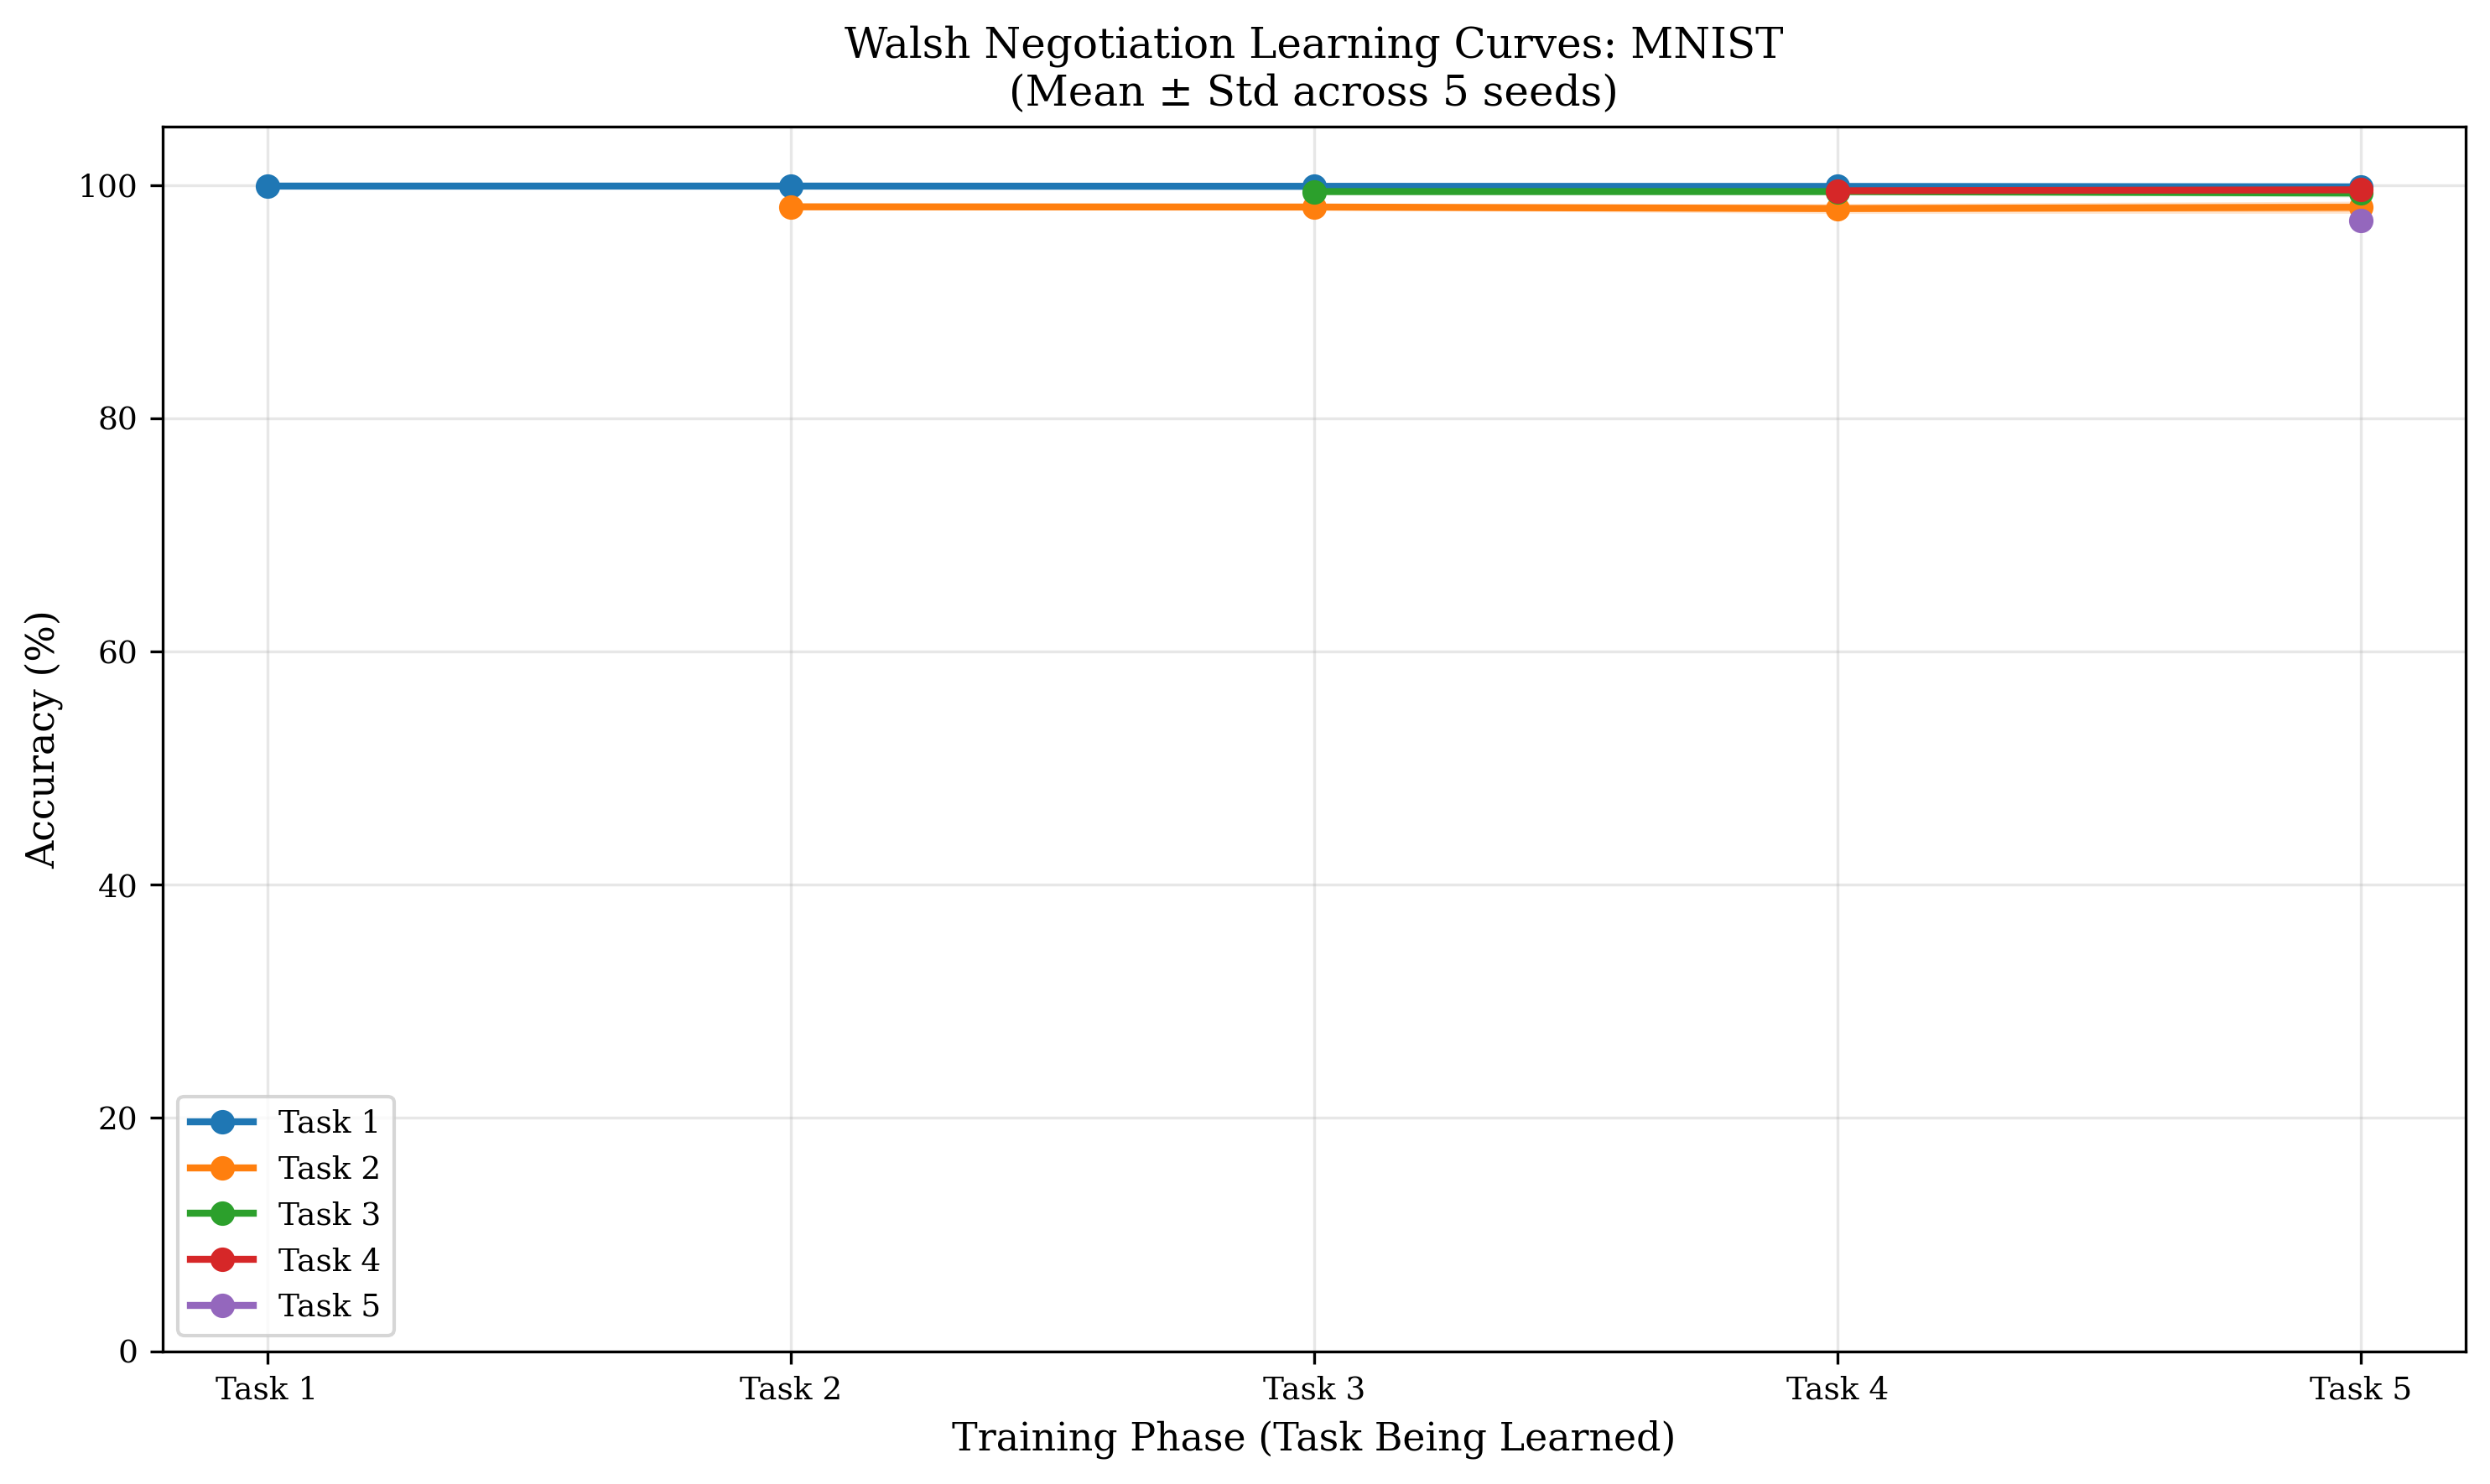
\includegraphics[width=\columnwidth]{walsh_learning_curves_mnist.png}
\caption{Walsh Negotiation learning curves on Split-MNIST showing task-by-task accuracy across 5 seeds.}
\label{fig:walsh_learning_curves_mnist}
\end{figure}

\begin{figure}[t]
\centering
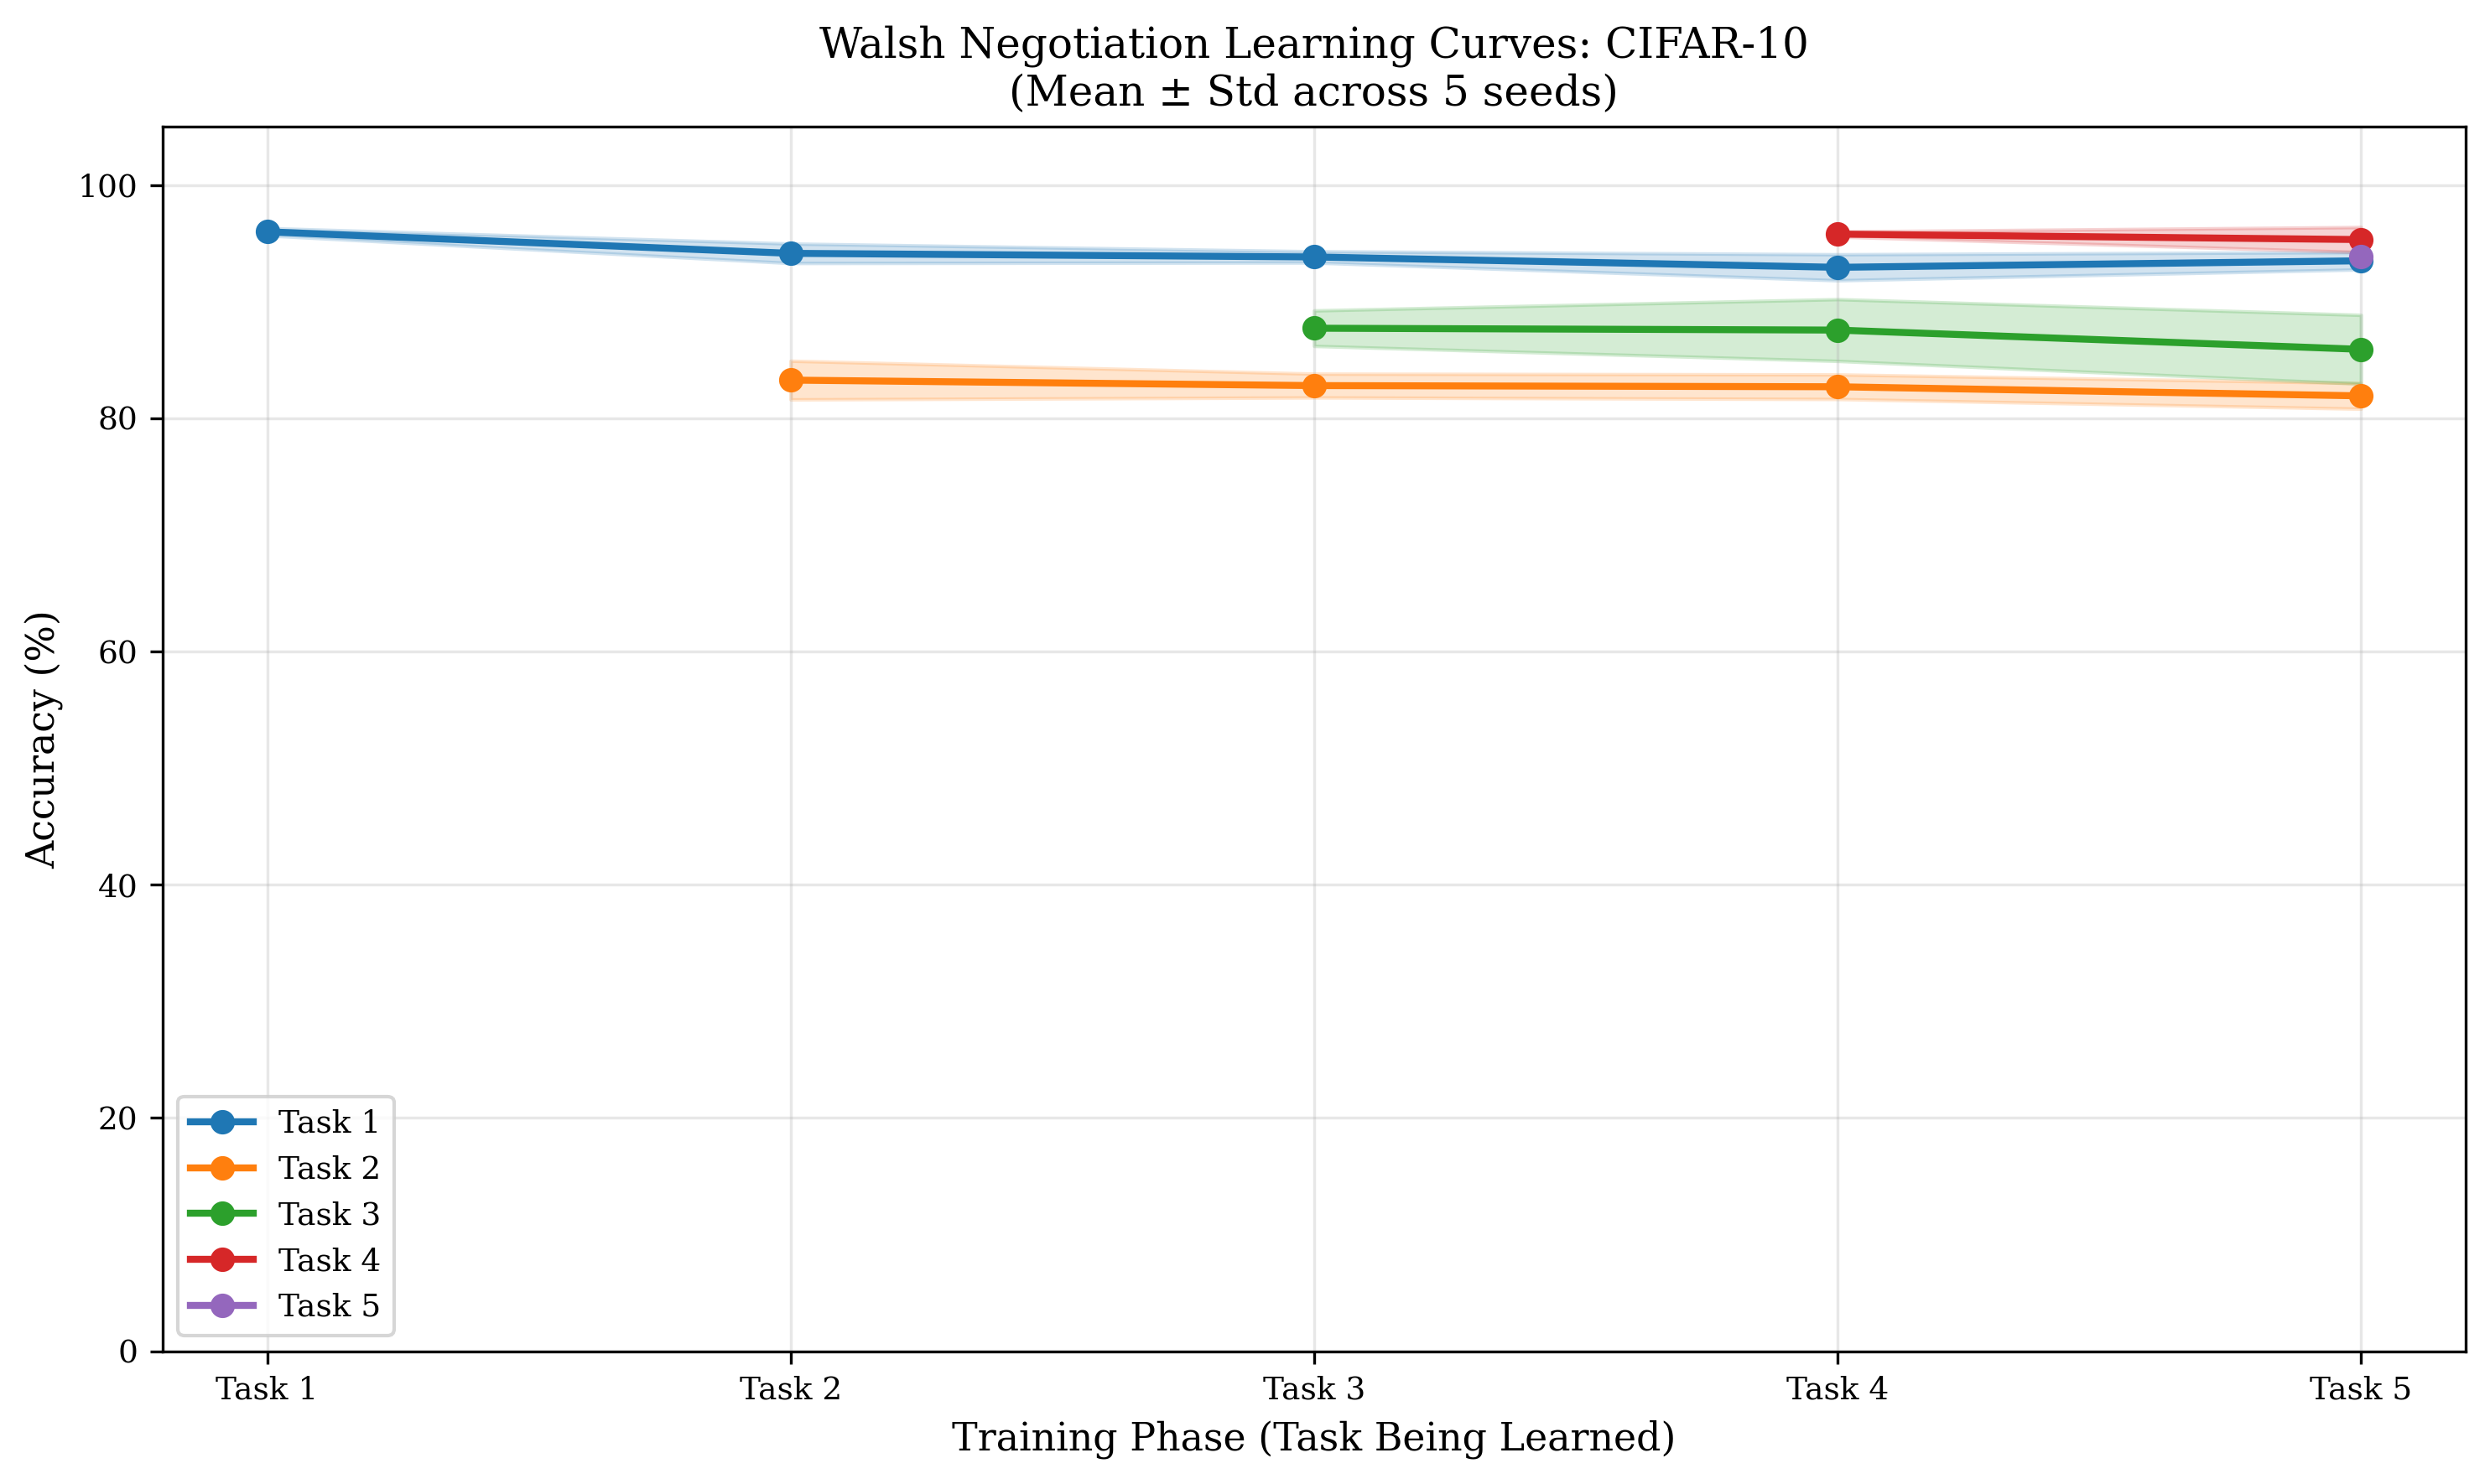
\includegraphics[width=\columnwidth]{walsh_learning_curves_cifar10.png}
\caption{Walsh Negotiation learning curves on Split-CIFAR-10 showing task-by-task accuracy across 5 seeds.}
\label{fig:walsh_learning_curves_cifar10}
\end{figure}

\begin{figure}[t]
\centering
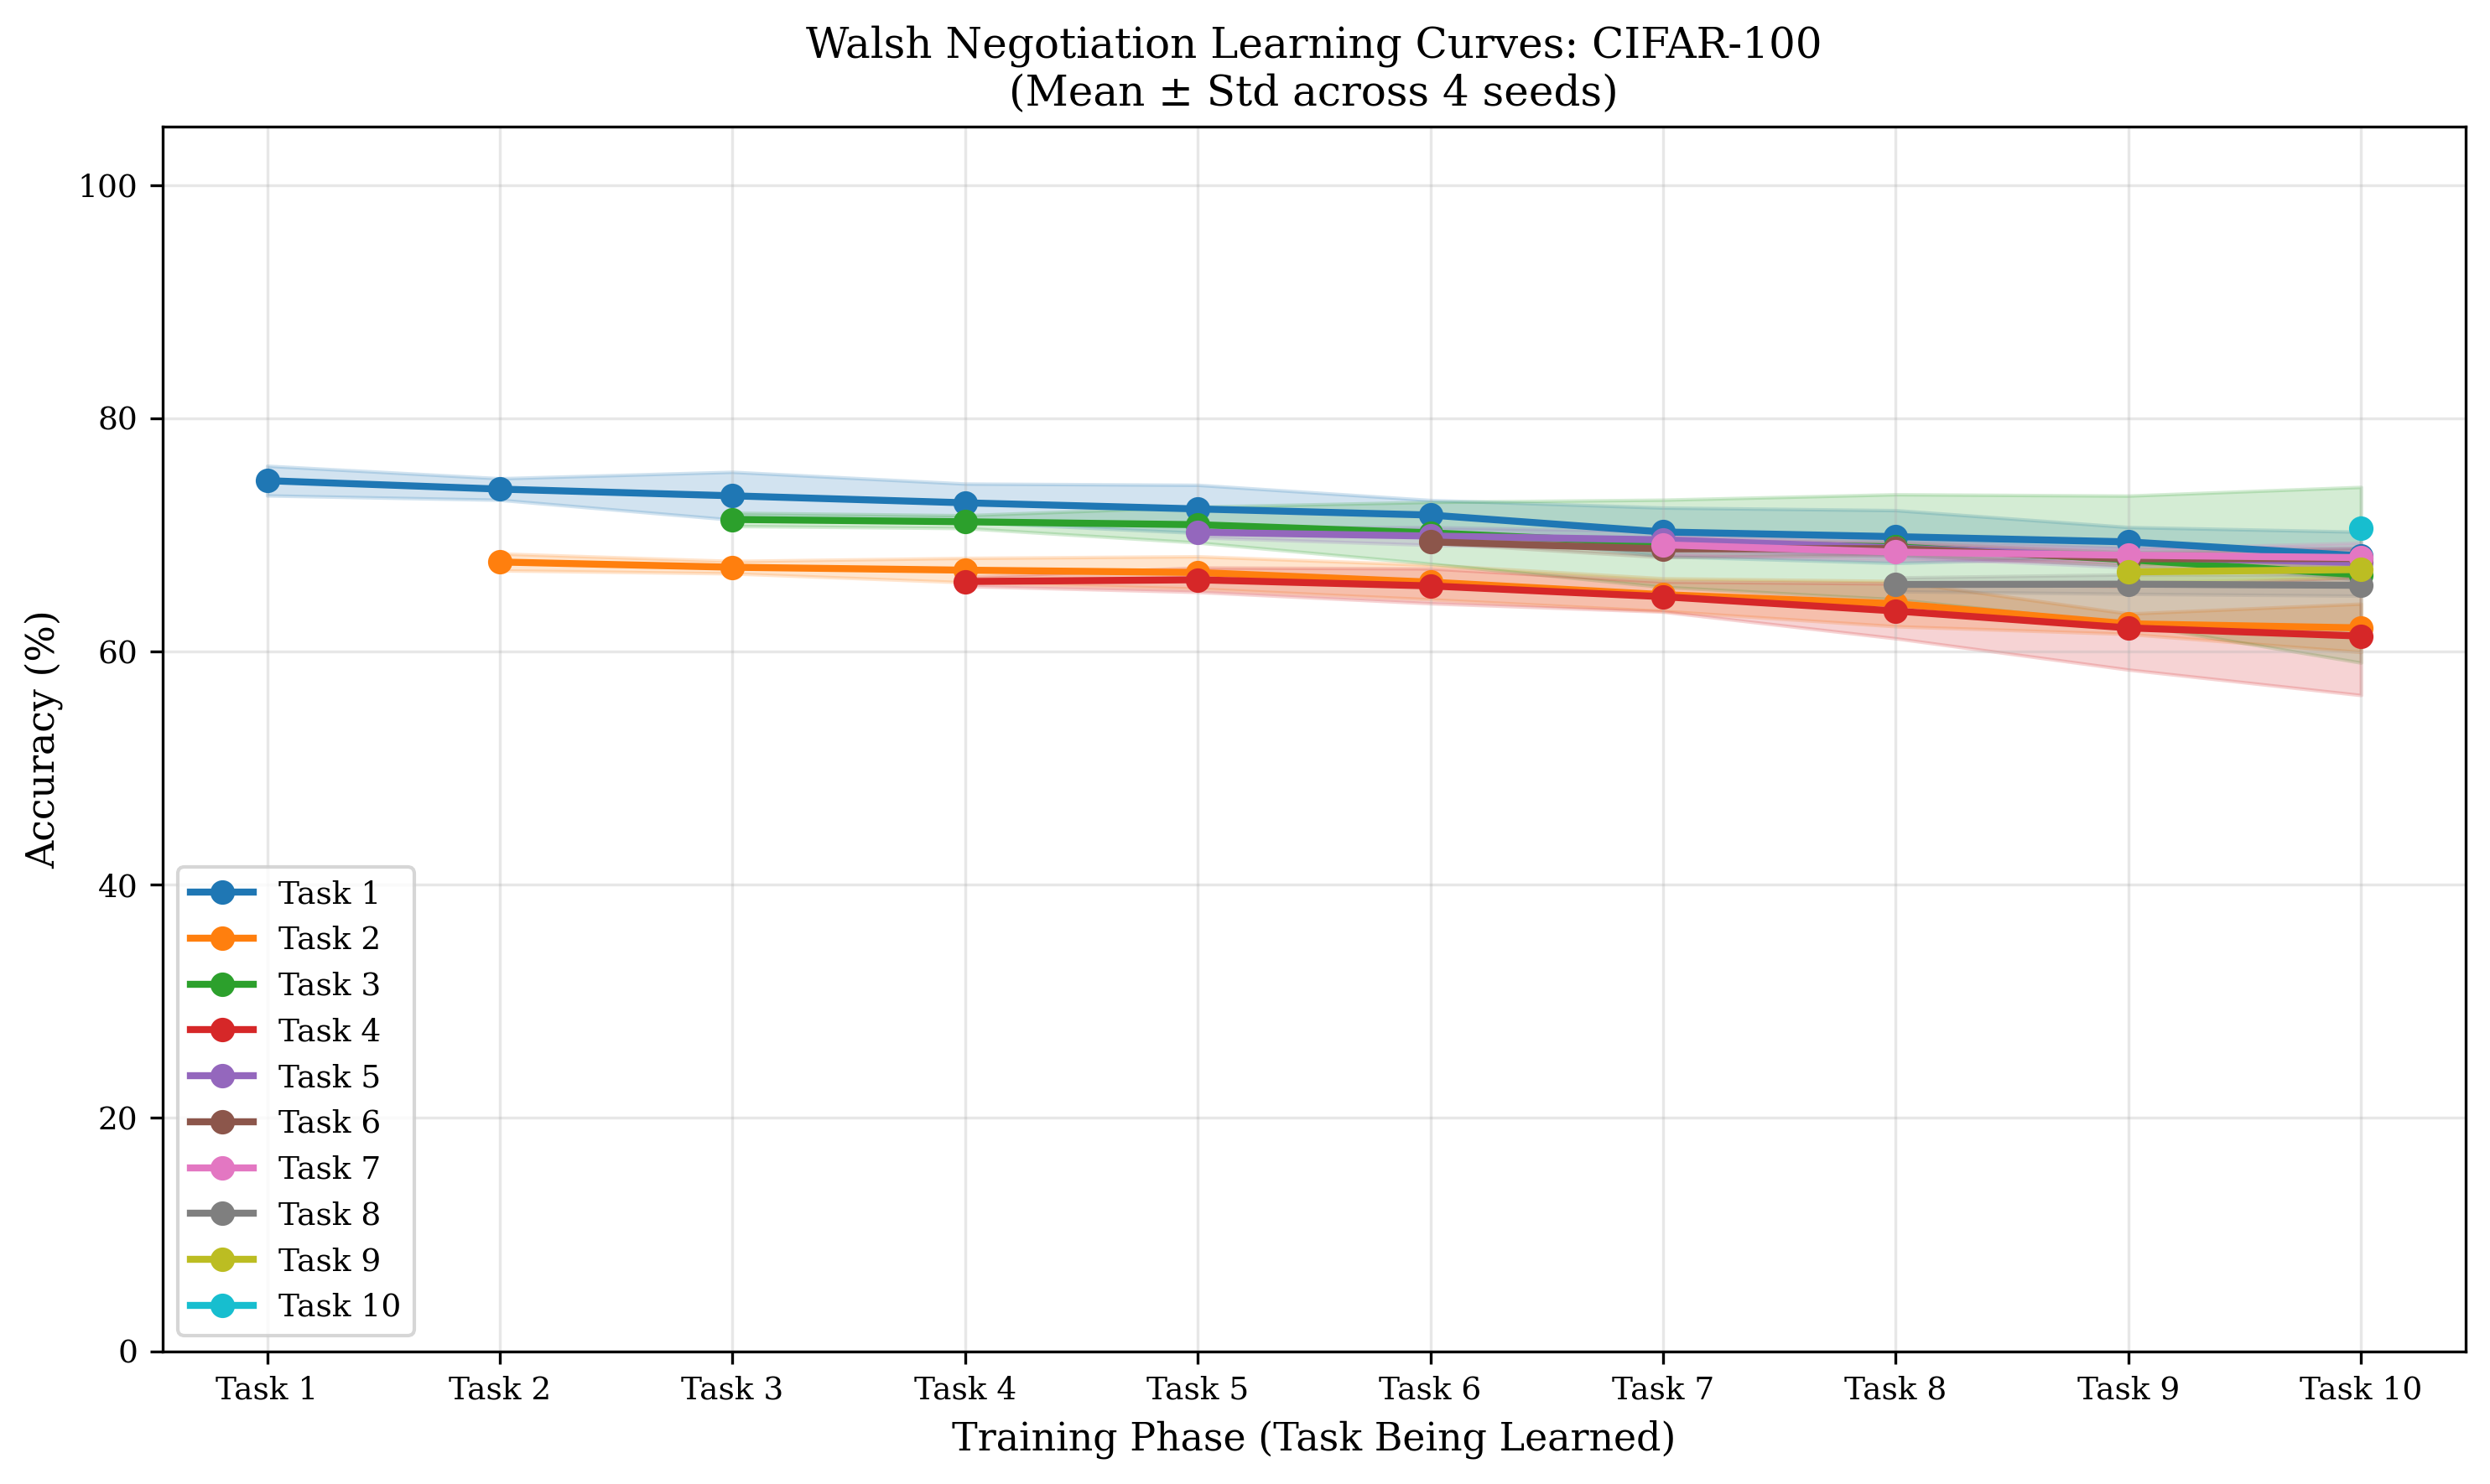
\includegraphics[width=\columnwidth]{walsh_learning_curves_cifar100.png}
\caption{Walsh Negotiation learning curves on Split-CIFAR-100 showing task-by-task accuracy across 5 seeds.}
\label{fig:walsh_learning_curves_cifar100}
\end{figure}

\begin{figure*}[t]
\centering
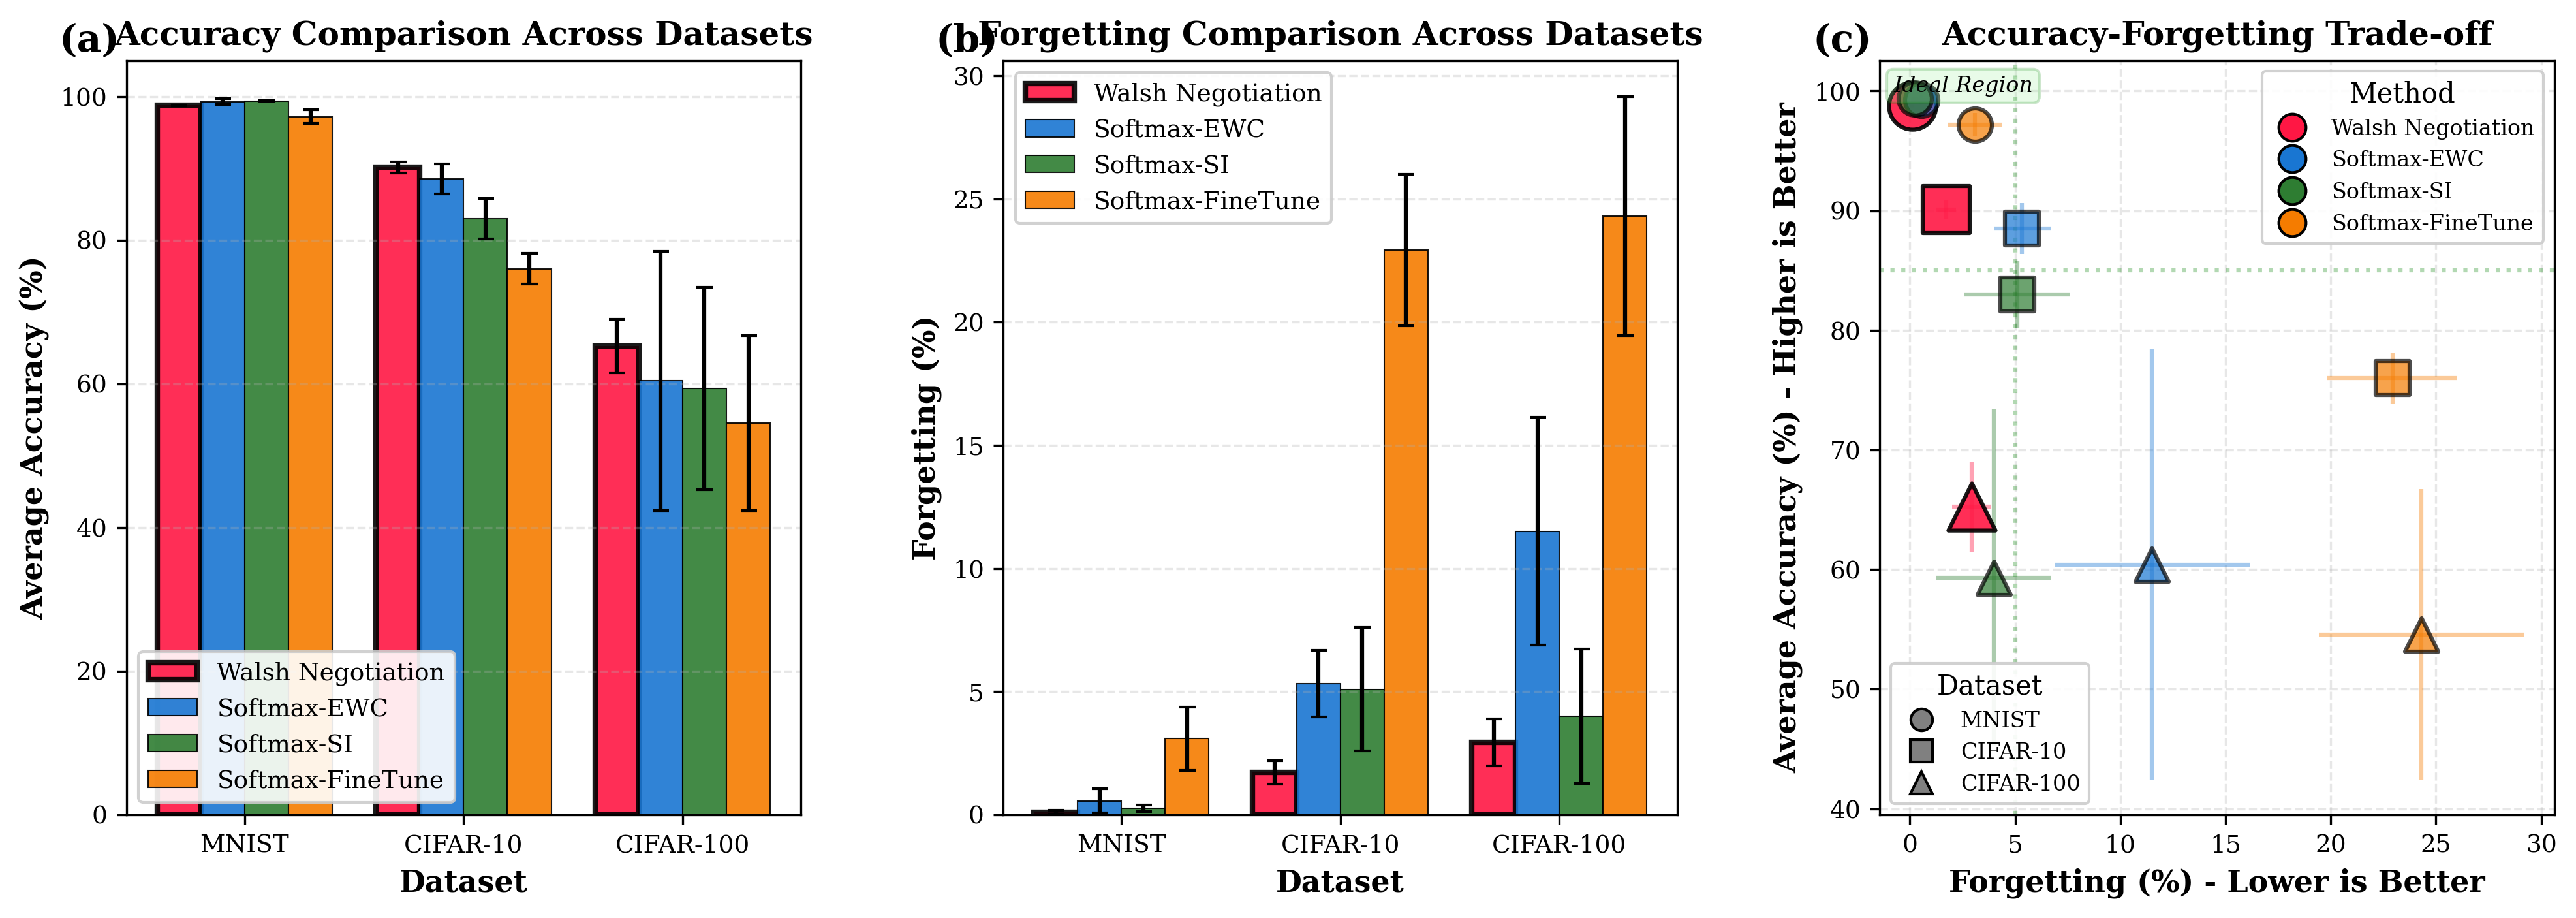
\includegraphics[width=0.7\textwidth]{cross_dataset_summary_walsh.png}
\caption{Cross-dataset summary comparing Walsh Negotiation with other methods on forgetting and accuracy metrics.}
\label{fig:cross_dataset_summary_walsh}
\end{figure*}

\subsection{Cross-dataset analysis}

Fig.~\ref{fig:cross_dataset_summary_walsh} visualizes the cross-dataset comparison of forgetting and accuracy metrics for Walsh Negotiation and other leading methods.

\begin{table}[h]
\centering
\caption{Forgetting comparison across datasets under default training schedules. Walsh Negotiation uses 50 epochs/task; other methods use 10 (MNIST) or 20 (CIFAR) epochs/task. See Tables~\ref{tab:equal_compute_cifar100}--\ref{tab:equal_compute_mnist} for iso-compute results.}
\label{tab:forgetting_trends}
\begin{tabular}{lcccc}
\toprule
Method & Ep./Task & MNIST & CIFAR-10 & CIFAR-100 \\
\midrule
Walsh-Negot. & 50 & \textbf{0.10\%} & \textbf{1.71\%} & \textbf{2.94\%} \\
Softmax-SI & 10/20 & 0.25\% & 5.48\% & 2.71\% \\
Softmax-EWC & 10/20 & 0.75\% & 5.70\% & 9.68\% \\
Softmax-FT & 10/20 & 2.46\% & 23.13\% & 25.86\% \\
Sigmoid-FT & 10/20 & 6.28\% & 18.48\% & 28.29\% \\
\bottomrule
\multicolumn{5}{l}{\scriptsize Note: Walsh uses 2.5--5$\times$ the per-task epochs of baselines.} \\
\multicolumn{5}{l}{\scriptsize At equal compute (50 ep.), SI forgetting is comparable:} \\
\multicolumn{5}{l}{\scriptsize 0.19\% (MNIST), 3.13\% (CIFAR-10), 3.17\% (CIFAR-100).}
\end{tabular}
\end{table}

\begin{table}[h]
\centering
\caption{CIFAR-10 stabilized schedule comparison. Walsh Negotiation uses its default (untuned) schedule with 50 epochs/task. All other methods use the tuned schedule with 20 epochs/task.}
\label{tab:cifar10_stabilized_comparison}
\begin{tabular}{lcc}
\toprule
Method & CIFAR-10 Forg. & Notes \\
\midrule
Walsh-Negot.$^\dagger$ & \textbf{1.71\%} & No tuning needed \\
LwF & 1.74\% & Tuned schedule \\
Softmax-EWC & 2.72\% & 52\% impr.\ vs.\ untuned \\
MAS & 3.56\% & Tuned schedule \\
Softmax-FT & 12.02\% & 48\% impr.\ vs.\ untuned \\
Softmax-SI & 13.20\% & Degr.\ vs.\ untuned \\
\bottomrule
\multicolumn{3}{l}{\scriptsize $^\dagger$Walsh Negotiation uses 50 epochs/task} \\
\multicolumn{3}{l}{\scriptsize with default (untuned) hyperparameters.}
\end{tabular}
\end{table}

\textbf{Consistent patterns across datasets:}
\begin{enumerate}
\item \textbf{Walsh Negotiation achieves the lowest forgetting at default epoch settings}: $0.10\%$ (MNIST), $1.71\%$ (CIFAR-10), $2.94\%$ (CIFAR-100). At equal compute (50 epochs), Walsh retains the lowest forgetting on all three datasets, though the margin over SI narrows substantially ($0.10\%$ vs.\ $0.19\%$ on MNIST, $1.71\%$ vs.\ $3.13\%$ on CIFAR-10, $2.94\%$ vs.\ $3.17\%$ on CIFAR-100).
\item \textbf{Walsh Negotiation provides inherent stability}: Achieves low variance ($<$\,1\% std) on all datasets without tuning, while other methods show moderate to high variance (1--6\% std) that can be reduced with dataset-specific optimization.
\item \textbf{At equal compute, SI is the strongest competitor}: SI benefits substantially from additional training epochs, achieving the highest accuracy on CIFAR-100 ($71.64\%$) and MNIST ($99.51\%$) at 50 epochs. On CIFAR-10, Walsh maintains a clear advantage.
\item \textbf{LwF and EWC benefit from dataset-specific tuning}: On stabilized CIFAR-10, LwF achieves $93.17\%$ accuracy with $1.74\%$ forgetting at only 20 epochs, surpassing Walsh on accuracy while using less compute. However, this requires dataset-specific hyperparameter optimization.
\item \textbf{EWC is fragile under extended training}: EWC collapses to random-chance accuracy at 50 epochs on both CIFAR benchmarks, revealing a fundamental limitation of Fisher-based regularization under extended training.
\item \textbf{Sigmoid paradigm helps only on MNIST}, with performance degradation on CIFAR datasets.
\end{enumerate}

\subsection{Sigmoid-SI failure analysis}
\label{sec:sigmoid_si_failure}

The complete failure of Sigmoid-SI warrants detailed investigation. We observe:

\begin{enumerate}
\item \textbf{Deterministic failure}: Zero variance across all 5 seeds indicates the failure is not due to random initialization but a fundamental algorithmic issue.

\item \textbf{Random guessing}: $49.33\%$ on MNIST (random = 50\%), $50.00\%$ on CIFAR-10 (random = 50\%), $10.00\%$ on CIFAR-100 (random = 10\%) confirms the model outputs near-uniform distributions.

\item \textbf{Gradient explosion}: Training logs reveal NaN gradients after Task 0, consistent with unbounded accumulation in path-integral importance.

\item \textbf{BCE-SI incompatibility}: Binary cross-entropy loss has unbounded gradients near 0 and 1, interacting poorly with the multiplicative importance weights in SI.
\end{enumerate}

This represents a \textbf{fundamental incompatibility} between sigmoid activations (BCE loss) and path-integral regularization (SI), rendering Sigmoid-SI unusable for continual learning without major algorithmic modifications.

\begin{figure}[t]
\centering
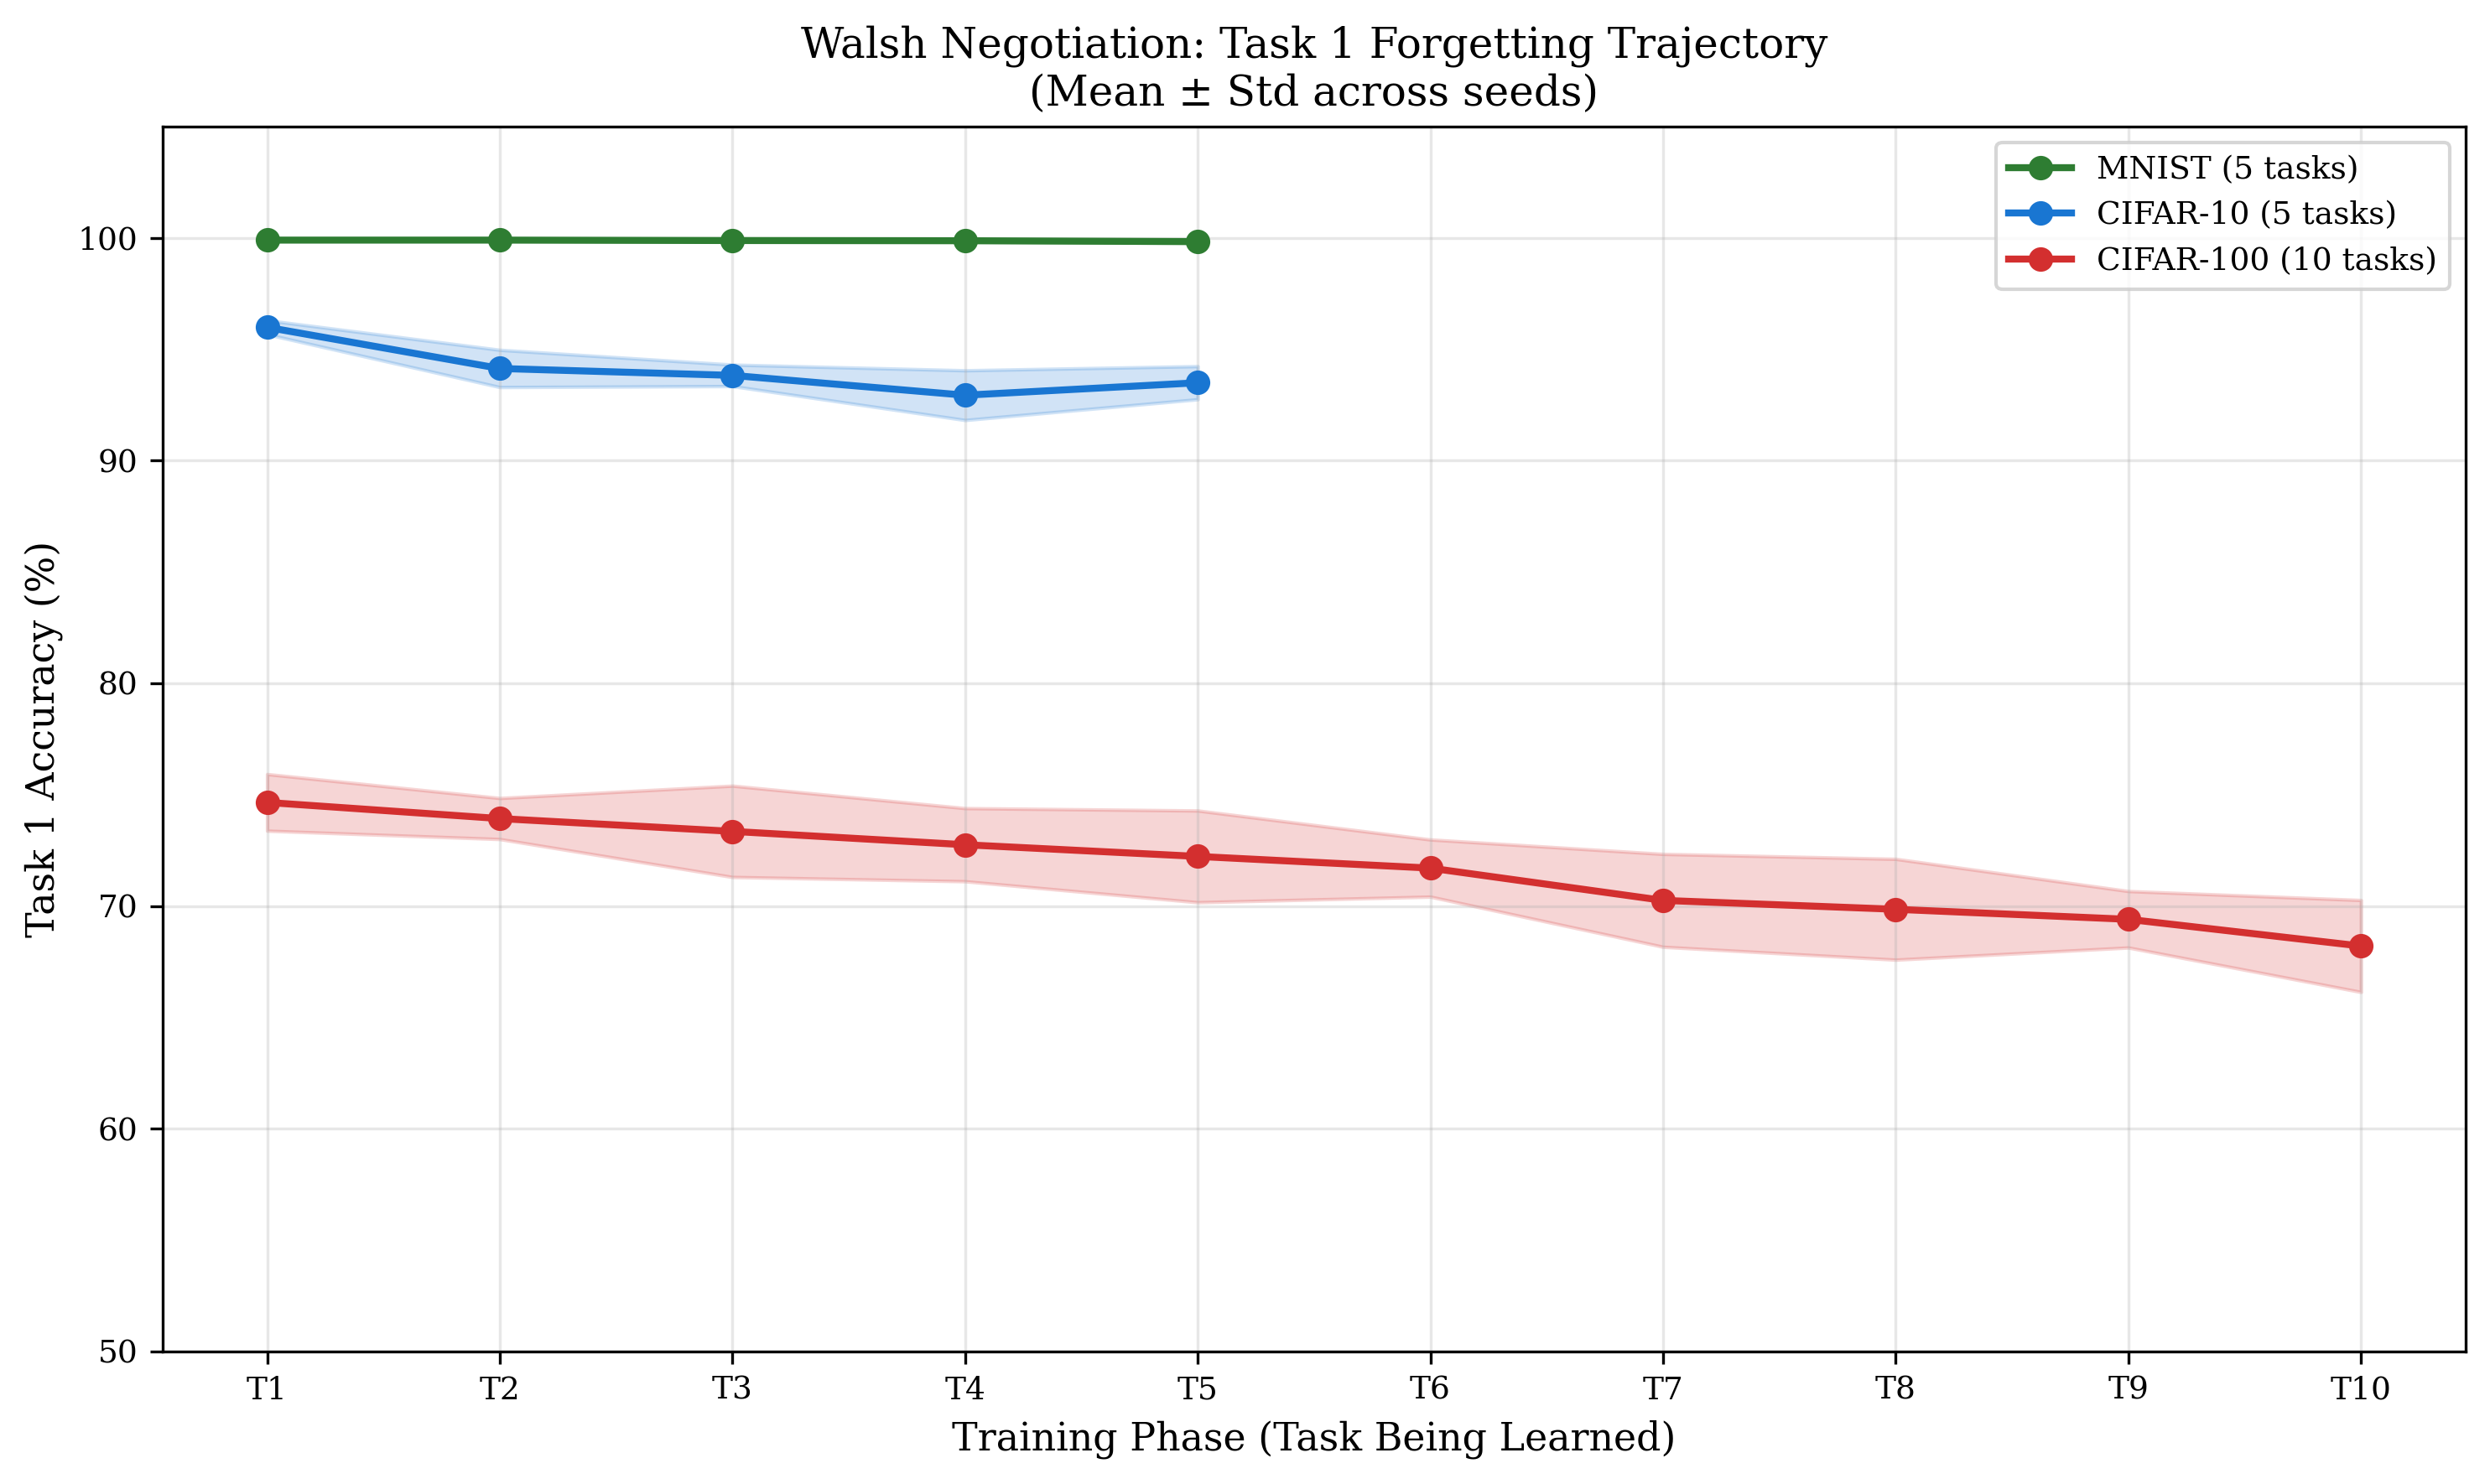
\includegraphics[width=\columnwidth]{walsh_forgetting_trajectory.png}
\caption{Task 1 accuracy degradation trajectory across datasets comparing Walsh Negotiation with other methods. Walsh Negotiation demonstrates superior retention of Task 1 performance as new tasks are learned, with minimal degradation on all three benchmarks (MNIST, CIFAR-10, CIFAR-100).}
\label{fig:walsh_forgetting_trajectory}
\end{figure}

\subsection{Variance analysis}

\begin{itemize}
\item \textbf{Untuned CIFAR-10:} Accuracy std 1--6\%, forgetting std 1--7\% (moderate variance for non-Walsh methods).
\item \textbf{Tuned CIFAR-10:} Accuracy std drops to approximately 1--5\% for LwF/EWC/MAS; forgetting std to $<$2\% for LwF/EWC and approximately 1.5\% for MAS; SI and Fine-Tune remain higher (approximately 1--3\% forgetting std, $>$2\% accuracy std); negotiation still shows high variance (approximately 5\% accuracy std, approximately 4--5\% forgetting std).
\item \textbf{MNIST/CIFAR-100:} Remain stable (accuracy std $<$3\%, forgetting std $<$4\%).
\item \textbf{Walsh Negotiation across all settings:} Consistently achieves the lowest variance among all methods (accuracy std $\leq$ 0.84\%, forgetting std $\leq$ 1.05\%), without any dataset-specific tuning.
\end{itemize}

\textbf{CIFAR-10 stability with tuning:} A CIFAR-10-specific schedule (lr 0.0025, weight decay 5e-4, multistep milestones 10/15, gradient clipping 5.0) reduces variance to approximately 1--3\% and improves forgetting to $<$4\% for EWC/MAS; LwF achieves $1.74\%$ forgetting with similar variance.

\section{Discussion}

\subsection{Walsh Negotiation: Strengths and limitations}

Walsh Negotiation~\cite{korhan2023negotiated} demonstrates several genuine strengths in our evaluation, but a fair assessment must also acknowledge where other methods excel.

\textbf{Genuine strengths:}

\textit{Robustness to extended training.} Walsh Negotiation is the only method in our comparison that maintains stable, low-forgetting performance across all datasets when trained for 50 epochs per task. EWC collapses to random-chance accuracy at 50 epochs on CIFAR-10 ($50.00\%$) and CIFAR-100 ($10.00\%$), FineTune degrades on MNIST, and even EWC degrades on MNIST (from $99.12\%$ to $96.04\%$). Walsh maintains consistent performance regardless of training duration, a practically important property.

\textit{Lowest variance across all settings.} Walsh Negotiation achieves the lowest standard deviation among all methods on every dataset: $0.07\%$ accuracy std on MNIST, $0.78\%$ on CIFAR-10, and $0.84\%$ on CIFAR-100. This means practitioners can rely on Walsh Negotiation to deliver predictable performance, whereas other methods may exhibit runs with substantially degraded results.

\textit{No dataset-specific tuning required.} Walsh Negotiation uses identical hyperparameters ($\alpha_0 = 0.5$, 50 epochs, lr = 0.01) across all three datasets, while the best-performing baselines require dataset-specific optimization. The stabilized CIFAR-10 schedule (Table~\ref{tab:cifar10_stable}) demonstrates that LwF and EWC can match or exceed Walsh's performance, but only with careful tuning of learning rate, weight decay, scheduler, and gradient clipping.

\textit{Clear victory on CIFAR-10 at equal compute.} At 50 epochs per task, Walsh achieves $90.11\%$ accuracy with $1.71\%$ forgetting, outperforming SI ($86.38\%$, $3.13\%$) on both metrics. This is the strongest evidence that the Walsh negotiation mechanism provides a genuine benefit beyond simply training longer.

\textit{Consistently lowest or near-lowest forgetting.} At equal compute, Walsh achieves the lowest forgetting on all three datasets ($2.94\%$ on CIFAR-100, $1.71\%$ on CIFAR-10, $0.10\%$ on MNIST), though the margin over SI is small on CIFAR-100 ($2.94\%$ vs.\ $3.17\%$) and MNIST ($0.10\%$ vs.\ $0.19\%$).

\textbf{Limitations revealed by equal-compute analysis:}

\textit{SI surpasses Walsh on accuracy on CIFAR-100 and MNIST.} At equal compute (50 epochs), SI achieves $71.64\%$ accuracy on CIFAR-100 vs.\ Walsh's $66.71\%$---a gap of nearly 5 percentage points with statistically comparable forgetting. On MNIST, SI achieves $99.51\%$ vs.\ Walsh's $98.75\%$. Walsh Negotiation is not the universally dominant method when baselines are given equal training time.

\textit{Higher epoch requirement.} The negotiation mechanism requires more epochs to converge because the negotiated targets are initially dominated by the model's poor early predictions, creating a bootstrapping problem that resolves gradually during training. This 2.5--5$\times$ epoch overhead is an inherent cost of the method.

\textit{LwF with tuning surpasses Walsh on CIFAR-10 accuracy.} On the stabilized CIFAR-10 schedule, LwF achieves $93.17\%$ accuracy with $1.74\%$ forgetting at only 20 epochs, while Walsh achieves $90.11\%$ with $1.71\%$ forgetting at 50 epochs. When dataset-specific tuning is available, knowledge distillation methods can be more compute-efficient.

\textbf{Mechanistic factors contributing to Walsh Negotiation's properties:}

\textit{Orthogonal target representations.} Walsh--Hadamard codes provide orthogonal, structured representations in a 128-dimensional space. This orthogonality ensures that target encodings for different classes are maximally separated, reducing interference between tasks during sequential learning. As noted by Korhan and {\"O}ner~\cite{korhan2023negotiated}, the use of Walsh codes ensures constant Hamming distance between all class pairs, which is a stronger structural guarantee than provided by one-hot encoding.

\textit{Balanced negotiation in structured space.} The negotiation parameter $\alpha_0 = 0.5$ blends true labels with model predictions in Walsh-encoded space rather than raw label space. This structured blending provides smoother gradient signals and avoids the noisy pseudo-label problem that plagues standard negotiation methods (Softmax-Negotiation: $38.56\%$ forgetting vs.\ Walsh: $2.94\%$ on CIFAR-100).

\textit{Implicit regularization through encoding.} The Walsh--Hadamard transformation acts as an implicit regularizer, projecting high-dimensional outputs into a structured subspace where task boundaries are more clearly defined. This may explain why Walsh Negotiation achieves low variance ($<$\,1\% std) without dataset-specific tuning.

\textit{Error correction properties.} Walsh--Hadamard codes have error-correcting properties commonly exploited in communications~\cite{olmez2021walsh}. In continual learning, this translates to robustness against gradient noise and task interference, enabling stable learning across all 50 epochs per task without collapse.

\textit{Dynamic plasticity scheduling.} The negotiation rate update formula $p(\alpha) = 1/(2\alpha - \alpha^2)$ from~\cite{korhan2023negotiated} ensures equal capacity allocation across tasks, preventing early tasks from monopolizing model capacity while maintaining sufficient plasticity for later tasks.

\subsection{Epoch count considerations and equal-compute analysis}
\label{sec:discussion_epochs}

An important aspect of our evaluation is that Walsh Negotiation uses 50 epochs per task, whereas baseline methods use 10 epochs (MNIST) or 20 epochs (CIFAR) in the default schedule. This difference arises because the negotiation mechanism requires additional training time to progressively refine the blended targets: early in training, the model's predictions are poor, so the negotiated targets are dominated by Walsh codes; as training progresses, the model's predictions improve, and the targets gradually shift to incorporate more of the model's own representations.

\textbf{To address this compute disparity, we conducted a comprehensive equal-compute analysis by training all baseline methods at 50 epochs per task} (Section~\ref{sec:equal_compute}). This analysis reveals several important findings:

\textbf{SI thrives with more epochs.} SI consistently benefits from extended training across all datasets: on CIFAR-100, accuracy improves from $63.08\%$ (20 epochs) to $71.64\%$ (50 epochs) with only a modest increase in forgetting ($2.71\%$ to $3.17\%$). On CIFAR-10, SI improves from $82.64\%$ to $86.38\%$ accuracy while forgetting \emph{decreases} from $5.48\%$ to $3.13\%$. On MNIST, SI improves from $99.37\%$ to $99.51\%$. SI's online importance accumulation mechanism appears well-suited to extended training.

\textbf{EWC collapses at 50 epochs.} On CIFAR-100, EWC accuracy drops from $66.06\%$ (20 epochs) to $10.00\%$ (50 epochs, random chance). On CIFAR-10, it drops from $88.11\%$ to $50.00\%$ (random chance). On MNIST, EWC degrades from $99.12\%$ to $96.04\%$. The Fisher information penalty accumulates over 50 epochs of gradient updates, causing the regularization term to dominate the learning signal and effectively freezing the model. This collapse is deterministic (zero variance across seeds on CIFAR-10 and CIFAR-100) and reveals a fundamental limitation of post-hoc Fisher-based importance estimation under extended training. Without hyperparameter retuning (e.g., reducing $\lambda$, recomputing Fisher information more frequently), EWC cannot be naively scaled to higher epoch counts.

\textbf{FineTune degrades on MNIST.} FineTune accuracy drops from $97.78\%$ (10 epochs) to $95.16\%$ (50 epochs) on MNIST, with forgetting increasing from $2.46\%$ to $5.76\%$, suggesting overfitting to later tasks.

\textbf{Walsh maintains stability.} Walsh Negotiation achieves consistent performance at 50 epochs across all datasets without collapse or degradation, confirming that the negotiation mechanism provides inherent stability under extended training. This robustness is a genuine and practically important advantage: practitioners do not need to worry about training too long, which is not the case for EWC or even FineTune.

\textbf{Honest assessment at equal compute:} When all methods are given 50 epochs, Walsh Negotiation achieves the lowest forgetting on all three datasets, but SI achieves substantially higher accuracy on CIFAR-100 (+4.93 pp) and moderately higher accuracy on MNIST (+0.76 pp). On CIFAR-10, Walsh wins on both metrics. The picture that emerges is that Walsh Negotiation is not universally superior, but rather the most \emph{robust and reliable} method---it never collapses, always achieves low forgetting, and does so with the lowest variance, but it can be outperformed on accuracy by SI when SI is given sufficient training time.

\subsection{Why does Softmax-SI outperform Softmax-EWC?}

While both SI and EWC are theoretically grounded regularization methods, SI consistently achieves lower forgetting than EWC in our experiments. We hypothesize three contributing factors:

\textbf{Online importance estimation:} SI computes importance online during training by accumulating $\sum g_i \Delta\theta_i$, capturing the actual optimization trajectory. EWC computes Fisher information post-hoc on the final parameters, potentially missing transient importance.

\textbf{Path-integral vs.\ point-estimate:} SI's path-integral formulation integrates importance over the entire learning trajectory, while EWC relies on a second-order Taylor approximation at a single point.

\textbf{No curvature assumption:} SI does not assume Gaussian posteriors or diagonal Fisher matrices, potentially capturing richer parameter importance structures.

Additionally, our equal-compute analysis reveals a practical advantage: SI's online importance mechanism scales gracefully with more training epochs, while EWC's post-hoc Fisher estimation causes catastrophic collapse at extended training durations.

These results align with Zenke et al.'s original findings~\cite{zenke2017continual}, now validated with rigorous statistical testing and extended to include epoch-scaling behavior.

\subsection{Why does sigmoid fail on complex datasets?}

The sigmoid paradigm (BCE loss) underperforms on CIFAR datasets for several reasons:

\textbf{Independent probabilities:} Sigmoid treats each class independently, losing inter-class competition that softmax provides. On CIFAR-100 with 10 classes per task, this leads to poorly calibrated probabilities.

\textbf{Optimization difficulty:} BCE loss has steeper gradients near 0 and 1, potentially causing optimization instability, especially with regularization methods that constrain parameter updates.

\textbf{Loss of inductive bias:} Softmax implicitly enforces a sum-to-one constraint, providing useful inductive bias. Sigmoid lacks this constraint, requiring the model to learn normalization from data alone.

However, sigmoid helps on MNIST's simple binary tasks (Sigmoid-Negotiation: $98.82\%$ vs.\ Softmax-Negotiation: $98.34\%$), suggesting it may be beneficial for truly binary classification scenarios.

\subsection{Why does Sigmoid-SI fail catastrophically?}

The complete failure of Sigmoid-SI ($10\%$ accuracy on CIFAR-100, zero variance) reveals a \textbf{fundamental mathematical incompatibility}:

\textbf{Gradient unboundedness:} BCE loss gradient $\nabla_{\theta} \mathcal{L}_{BCE} = \sigma(z) - y$ can become large when $\sigma(z)$ is far from $y$. Combined with SI's importance accumulation $\omega_i \propto \sum |g_i \Delta\theta_i|$, this causes unbounded importance growth.

\textbf{Multiplicative drift:} SI regularizes with $\mathcal{L}_{SI} = \frac{\lambda}{2} \sum_i \omega_i (\theta_i - \theta^*_i)^2$. When $\omega_i \to \infty$, parameters freeze, preventing learning on new tasks.

\textbf{NaN propagation:} Training logs confirm NaN gradients after Task 0, causing immediate collapse to random guessing on subsequent tasks.

This failure is \textbf{deterministic} (zero variance across seeds) and \textbf{not addressable through hyperparameter tuning alone}; it would require major algorithmic modifications such as gradient clipping, logarithmic importance scaling, or per-task normalization.

\subsection{Implications for practitioners}

Our equal-compute analysis and tuning experiments provide nuanced, evidence-based guidance:

\textbf{When tuning budget is limited, use Walsh Negotiation~\cite{korhan2023negotiated}}: Walsh requires no dataset-specific tuning and achieves consistently low forgetting across all benchmarks with the lowest variance of any method. It is the safest default choice, particularly when the training duration cannot be precisely controlled or when predictability is paramount.

\textbf{When compute is limited and accuracy is critical, consider tuned LwF or EWC}: On CIFAR-10, LwF with a tuned schedule achieves $93.17\%$ accuracy and $1.74\%$ forgetting at only 20 epochs, surpassing Walsh ($90.11\%$, $1.71\%$) on accuracy at 40\% of the compute. EWC with tuning achieves $91.62\%$ accuracy with $2.72\%$ forgetting. However, these results require dataset-specific hyperparameter search.

\textbf{When ample compute is available, SI is a strong alternative on CIFAR-100 and MNIST}: At 50 epochs, SI achieves the highest accuracy on CIFAR-100 ($71.64\%$) and MNIST ($99.51\%$) with forgetting comparable to Walsh. SI requires no hyperparameter tuning for the training schedule (it uses the same default hyperparameters across epoch counts), but note that it exhibits higher variance than Walsh.

\textbf{For CIFAR-10 specifically, Walsh Negotiation is the strongest untuned method}: At equal compute, Walsh wins on both accuracy and forgetting, making it the recommended choice when CIFAR-10-like datasets are encountered.

\textbf{Avoid sigmoid activations} on complex datasets (CIFAR-level and above). Only consider for simple binary classification scenarios.

\textbf{Never use Sigmoid-SI}: Fundamental incompatibility renders it unusable.

\textbf{Be cautious with EWC at high epoch counts}: EWC collapses at 50 epochs on CIFAR benchmarks. If extended training is needed, prefer SI or Walsh Negotiation.

\subsection{Limitations}

Our study has several limitations:

\textbf{Task-incremental setting only:} We evaluate multi-head architectures with task IDs at test time. Class-incremental (single-head) and domain-incremental settings remain unexplored for the methods compared here.

\textbf{Epoch count trade-off:} Walsh Negotiation inherently requires more epochs than standard methods due to its self-referential target generation mechanism. While we provide equal-compute comparisons, a more comprehensive analysis varying epoch counts from 10 to 100 for all methods would further clarify the accuracy--compute trade-off frontier.

\textbf{Limited replay-based methods:} We focus on regularization approaches. Experience replay methods (iCaRL, A-GEM) may achieve different forgetting-accuracy trade-offs.

\textbf{No architecture search:} We use standard architectures (MLP for MNIST, ResNet-18 for CIFAR). Dynamic architectures (PackNet, HAT) may offer orthogonal benefits.

\textbf{Fixed hyperparameters for 50-epoch baselines:} When running baselines at 50 epochs, we use the same hyperparameters as the 20-epoch runs. Methods like EWC might benefit from reduced $\lambda$ values or Fisher recomputation strategies at higher epoch counts. Our results represent what happens when methods are naively scaled, not the best achievable performance with epoch-specific tuning.

\textbf{CIFAR-10 stabilization as case study only:} The tuned CIFAR-10 schedule uses 5 seeds; broader sweeps and ablation coverage remain future work.

\section{Conclusion}

We present a comprehensive multi-seed analysis of continual learning methods under the \textbf{task-incremental} setting, complementing the original class-incremental evaluation by Korhan and {\"O}ner~\cite{korhan2023negotiated}. Our study includes the first equal-compute comparison (50 epochs per task for all methods) in the Walsh Negotiation literature, providing an honest assessment of each method's strengths and limitations.

Walsh Negotiation achieves the lowest forgetting on all three datasets at equal compute: $0.10\% \pm 0.07\%$ on MNIST, $1.71\% \pm 0.44\%$ on CIFAR-10, and $2.94\% \pm 1.05\%$ on CIFAR-100, with the lowest variance among all methods tested. On CIFAR-10, Walsh achieves the best overall performance at equal compute, outperforming SI on both accuracy ($90.11\%$ vs.\ $86.38\%$) and forgetting ($1.71\%$ vs.\ $3.13\%$). However, on CIFAR-100, SI at 50 epochs achieves substantially higher accuracy than Walsh ($71.64\%$ vs.\ $66.71\%$) with comparable forgetting ($3.17\%$ vs.\ $2.94\%$), and on MNIST, SI leads on accuracy ($99.51\%$ vs.\ $98.75\%$) with near-identical forgetting ($0.19\%$ vs.\ $0.10\%$).

Walsh Negotiation is best characterized as the most \textbf{robust and reliable} continual learning method in our comparison: it never collapses under extended training (unlike EWC, which drops to random-chance accuracy at 50 epochs on both CIFAR benchmarks), requires no dataset-specific hyperparameter tuning (unlike LwF and the stabilized EWC schedule), and achieves the lowest variance across all settings. These properties make it a strong default choice when predictability and ease of deployment matter more than maximizing accuracy on a specific benchmark.

Among traditional regularization methods, Synaptic Intelligence with softmax activations (Softmax-SI) emerges as a powerful alternative that scales well with additional training epochs. At equal compute, SI achieves the highest accuracy on CIFAR-100 ($71.64\%$) and MNIST ($99.51\%$) with forgetting comparable to Walsh. For CIFAR-10, a stabilized tuning schedule yields competitive results for LwF ($93.17\%$ accuracy, $1.74\%$ forgetting) at only 20 epochs, demonstrating that dataset-specific optimization can match or exceed Walsh's accuracy at lower compute cost.

We additionally explore a sigmoid activation paradigm, finding benefits only on simple datasets (MNIST) but severe degradation on complex benchmarks (CIFAR). We identify a fundamental incompatibility between sigmoid activations and path-integral regularization (SI), resulting in deterministic failure ($10\%$ accuracy with zero variance across seeds).

Our rigorous multi-seed validation provides confidence in reproducibility and establishes clear recommendations for practitioners: \textbf{use Walsh Negotiation as the default method} when hyperparameter tuning budget is limited and predictable, low-forgetting performance is needed across diverse datasets; use Softmax-SI when ample compute is available and accuracy is the priority (particularly on CIFAR-100); use LwF or tuned EWC when dataset-specific optimization is feasible and compute efficiency matters. Avoid sigmoid activations on complex datasets and never use Sigmoid-SI.

\textbf{Future work} should investigate: (1) class-incremental evaluation without task IDs for Walsh Negotiation, (2) integration with replay methods, (3) deeper theoretical analysis of why Walsh--Hadamard codes provide superior task separation, (4) extension to higher-dimensional Walsh codes (256, 512) for more complex datasets, (5) epoch-specific hyperparameter tuning for baselines (e.g., reduced $\lambda$ for EWC at 50 epochs) to establish an optimal accuracy--compute frontier for each method, (6) analysis of optimal negotiation parameter $\alpha_0$ across different dataset characteristics, and (7) gradient clipping or log-scaling strategies for Sigmoid-SI recovery.

\section*{Declaration of competing interest}

The authors declare that they have no known competing financial interests or personal relationships that could have appeared to influence the work reported in this paper.

\section*{Declaration of generative AI and AI-assisted technologies in the writing process}

During the preparation of this work the authors used Claude (Anthropic) for assistance with code development, data analysis automation, and manuscript formatting. The authors reviewed and edited all AI-assisted output and take full responsibility for the content of the publication.

\section*{CRediT authorship contribution statement}

\textbf{Salih \c{C}olako\u{g}lu:} Methodology, Software, Investigation, Formal analysis, Writing -- original draft, Writing -- review \& editing.
\textbf{Nuri Korhan:} Conceptualization, Methodology, Supervision, Writing -- review \& editing.
\textbf{Mustafa Onat:} Supervision, Writing -- review \& editing.

\section*{Acknowledgments}

This research was supported by [grant information to be added]. Computational resources were provided by [institution/computing facility to be added].

\section*{Data availability}

All datasets used in this study (MNIST, CIFAR-10, CIFAR-100) are publicly available. Code and experimental scripts are available at [URL to be added].

\bibliographystyle{elsarticle-num}
\bibliography{references}

\section*{Author Biographies}

\begin{biography}[salih_colakoglu.png]{Salih \c{C}olako\u{g}lu}
received the B.S. degree in electronic and communication engineering from Y{\i}ld{\i}z Technical University, Istanbul, Turkey, in 2014, and the M.S. degree in electrical and electronics engineering from Marmara University, Istanbul, in 2022, where his thesis focused on the design, fabrication, and characterization of a novel Lamb wave device. He is currently pursuing the Ph.D. degree in electrical and electronics engineering at Marmara University, under the supervision of Prof.\ Dr.\ Mustafa Onat.

Since 2020, he has been a Research Assistant with the Department of Electrical and Electronics Engineering, Marmara University. From 2012 to 2014, he was the Co-Founder and CEO of Teslaref Engineering, Istanbul, developing high-tech information systems and smart electronic devices. From 2014 to 2025, he served as the General Coordinator at Kodar Bili\c{s}im, Istanbul. His prior research was conducted at the Sabanc{\i} University Nanotechnology Research and Application Center (SUNUM) Laboratory, in collaboration with T\"{U}B\.{I}TAK ARDEB, focusing on RF MEMS resonators, acoustic plate waves, and micro/nanofabrication.

His current research interests include deep learning, continual learning, catastrophic forgetting mitigation, Walsh--Hadamard codes, structured negotiation paradigms for neural networks, embedded systems, and signal processing. ORCID: 0000-0002-2180-5073.
\end{biography}

\begin{biography}[nuri_korhan.png]{Nuri Korhan}
received the M.Sc. and Ph.D. degrees in mechatronics engineering from Istanbul Technical University, Istanbul, Turkey, in 2015 and 2023, respectively. His doctoral thesis focused on the classification of ten different motor imagery EEG signals using deep neural networks.

From 2013 to 2023, he was a Research Assistant with Istanbul Technical University, where he developed and implemented neural network models for brain--computer interfaces, computer vision applications, and embedded systems.

His research interests include deep learning, continual learning, negotiated representations, brain--computer interfaces, and motor imagery EEG classification. He introduced the negotiation paradigm for machine learning and has authored publications on neural network-based signal classification. ORCID: 0000-0003-4351-2885.
\end{biography}

\begin{biography}[mustafa_onat.jpg]{Mustafa Onat}
received the B.Sc. degree in electrical and electronics engineering from Middle East Technical University, Ankara, Turkey, in 1988, and the M.Sc. and Ph.D. degrees in computer-control engineering from Marmara University, Istanbul, Turkey, in 1996 and 2001, respectively.

From 1991 to 1994, he was an Instructor at Siirt University Vocational School. In 1994, he joined Marmara University as a Research Assistant with the Technical Education Faculty. He was promoted to Associate Professor in 2010 and transferred to the Faculty of Engineering in 2011, where he currently serves as a Professor with the Department of Electrical and Electronics Engineering, Control Systems Division.

His research interests include control systems, power electronics, neural networks, fault diagnosis, and intelligent systems. He has supervised numerous graduate theses and contributed to projects aligned with sustainable energy and smart systems. ORCID: 0000-0003-4304-3361.
\end{biography}

\end{document}
